\documentclass[10pt,a4paper]{article}
\newcommand{\runningtitle}{Neural topic scores in diabetic foot ulcer research}
\usepackage[margin=15mm,top=16mm,bottom=17mm,headheight=12pt,headsep=5mm,footskip=9mm]{geometry}
\usepackage{fontspec}
\setmainfont{TeX Gyre Termes}
\setsansfont{Arial}
\usepackage{amsmath,amssymb,mathtools,bm}
\usepackage{unicode-math}
\setmathfont{TeX Gyre Termes Math}
\usepackage{graphicx,booktabs,array,tabularx,longtable}
% Keep captions visually separated from their artwork/table rules, while
% retaining a compact single-column manuscript.  The same defaults are used
% by both papers so appendix tables and main-text figures do not drift apart.
\usepackage[font=small,labelfont=normalfont,labelsep=period,skip=8pt]{caption}
\usepackage{flafter,placeins,needspace}
\usepackage[sort&compress,numbers]{natbib}
\usepackage[unicode,colorlinks=true,linkcolor=black,citecolor=black,urlcolor=black]{hyperref}
% longtable 4.24 uses infinitely shrinkable glue before a kernel box split.
% Backport the upstream 4.25 finite-shrink fix (latex3/latex2e issue 1907)
% locally. etoolbox is already loaded by hyperref; no runtime/package changes.
% Patch both nested vbox branches. Already-fixed versions are left unchanged.
\makeatletter
\patchcmd{\LT@output}{\vss}{\vskip\z@\@plus1fil\@minus\normalbaselineskip}{}{}
\patchcmd{\LT@output}{\vss}{\vskip\z@\@plus1fil\@minus\normalbaselineskip}{}{}
\makeatother
\usepackage{xcolor,microtype,titlesec,enumitem,fancyhdr}
\usepackage{bookmark}
\hypersetup{pdfcreator={XeLaTeX},pdfauthor={Zeyu Fu}}
\graphicspath{{figures/}}
\setlength{\parindent}{1em}
\setlength{\parskip}{1pt plus .4pt}
\linespread{1.02}
\setlength{\textfloatsep}{12pt plus 2pt minus 1pt}
\setlength{\floatsep}{10pt plus 2pt minus 1pt}
\setlength{\intextsep}{12pt plus 2pt minus 1pt}
\renewcommand{\topfraction}{.94}
\renewcommand{\bottomfraction}{.88}
\renewcommand{\textfraction}{.06}
\renewcommand{\floatpagefraction}{.78}
\setcounter{topnumber}{3}
\setcounter{bottomnumber}{2}
\setcounter{totalnumber}{4}
\setlength{\abovedisplayskip}{4pt plus 1pt minus 2pt}
\setlength{\belowdisplayskip}{4pt plus 1pt minus 2pt}
\setlength{\abovedisplayshortskip}{2pt plus 1pt}
\setlength{\belowdisplayshortskip}{3pt plus 1pt}
\titlespacing*{\section}{0pt}{8pt plus 1pt minus 2pt}{3pt}
\titlespacing*{\subsection}{0pt}{6pt plus 1pt minus 1pt}{2pt}
\titleformat{\section}{\large\bfseries}{\thesection}{.6em}{}
\titleformat{\subsection}{\normalsize\bfseries}{\thesubsection}{.6em}{}
\setlist{nosep,leftmargin=1.7em,topsep=4pt}
\setlength{\bibsep}{1.5pt}
\renewcommand{\bibfont}{\small\let\emph\textnormal}
\setlength{\tabcolsep}{4pt}
% Longtable captions sit above the first rule.  These pre/post skips prevent
% adjacent appendix tables from reading as one continuous table while still
% allowing a continued table head to remain visually attached to its rows.
\setlength{\LTpre}{8pt plus 2pt minus 1pt}
\setlength{\LTpost}{8pt plus 2pt minus 1pt}
\setlength{\LTcapwidth}{\textwidth}
\captionsetup[figure]{skip=8pt}
\captionsetup[table]{skip=8pt}
\captionsetup[longtable]{font=footnotesize,skip=8pt}
\renewcommand{\arraystretch}{1.12}
\setlength{\emergencystretch}{1.2em}
\widowpenalty=10000
\clubpenalty=10000
\raggedbottom
\pagestyle{fancy}
\fancyhf{}
\fancyhead[L]{\sffamily\fontsize{8}{10}\selectfont\runningtitle}
\fancyfoot[C]{\small\thepage}
\renewcommand{\headrulewidth}{.25pt}
\newcommand{\papertitle}[1]{\thispagestyle{plain}\begin{center}\vspace*{-5mm}{\fontsize{19}{22}\selectfont\bfseries #1\par}\vspace{2mm}{\normalsize Zeyu Fu\par}\end{center}\vspace{-2mm}}
\newcommand{\paperfigure}[3]{\begin{figure}[!htbp]\centering\includegraphics[width=\linewidth]{#1.pdf}\caption{#3}\label{#2}\end{figure}}
\newcommand{\supplement}{\FloatBarrier\section*{Supplementary methods and numerical results}\addcontentsline{toc}{section}{Supplementary methods and numerical results}\setcounter{section}{0}\setcounter{table}{0}\setcounter{equation}{0}\renewcommand{\thesection}{S\arabic{section}}\renewcommand{\thetable}{S\arabic{table}}\renewcommand{\theequation}{S\arabic{equation}}\renewcommand{\theHsection}{supp.\arabic{section}}\renewcommand{\theHtable}{supp.\arabic{table}}\renewcommand{\theHequation}{supp.\arabic{equation}}}
\newcolumntype{L}{>{\raggedright\arraybackslash}X}
\newcommand{\doi}[1]{\href{https://doi.org/#1}{doi: #1}}
\newcommand{\E}{\mathbb{E}}
\newcommand{\R}{\mathbb{R}}
\newcommand{\ind}{\mathbf{1}}

\hypersetup{pdftitle={Neural topic modelling of fibroblast measurements and diabetic foot ulcer healing: a patient-level audit}}

\title{Neural topic modelling of fibroblast measurements and diabetic foot ulcer healing: a patient-level audit}
\author{Zeyu Fu$^{1,*}$\\[3pt]\small $^1$State Key Laboratory of Trauma and Chemical Poisoning,\\\small Institute of Combined Injury, Chongqing Engineering Research Center for Nanomedicine,\\\small College of Preventive Medicine, Army Medical University, Chongqing, China\\\small $^*$Correspondence: \texttt{fuzeyu09@gmail.com}; \texttt{fuzeyu99@126.com}}\date{}
\vfuzz=1pt
\begin{document}
\maketitle
\begin{abstract}
A high mean of a cellular programme need not indicate stronger expression within cells. We audited a frozen topic measurement and its association with diabetic-foot-ulcer healing in 11 patients; amputation was not an evaluated endpoint. The 15-topic model represented 76,461 cells from 25 foot-skin specimens and 20 patients. Decomposition, technical perturbations, refits and excluded intact-skin specimens evaluated the measurement. Prevalence accounted for 88\% of between-specimen variance in the fibroblast mean and 89\% between patients, with additional within-bin and covariance terms. High-scoring fibroblasts occurred in 9 of 11 ulcer patients and 2 of 15 intact foot-skin donors. Paired foot--forearm samples mixed ulcers with intact foot skin, limiting anatomical interpretation. Healing contrasts for the fibroblast mean, high-score fraction and composition were 0.0892, 0.1514 and 0.0708; all intervals included zero. Topic-selection adjustment gave probabilities of 0.785, 0.609 and 0.955 for the three discovery readouts. Selecting the topic within cross-validation gave areas under the receiver operating characteristic curve of 0.39--0.57, conditional on the discovery-trained encoder. Fifteen refits retained the direction but none reached \(p<0.05\). These calculations describe a prevalence-dominated readout without establishing a unique biological state or healing prediction.
\end{abstract}
\noindent\textbf{Keywords:} topic models; construct validity; fibroblasts; wound healing; CHI3L1; patient-level inference.

\section{Introduction}
Diabetic foot ulcers develop in tissue where neuropathy, vascular impairment, inflammation and repeated injury can coexist. Closure does not remove the risk of recurrence, making it important to understand which tissue measurements describe the current wound and which might inform its subsequent course \citep{armstrong2017,wilkinson2020}. Single-cell profiling has identified fibroblast-associated programmes that differ between healing groups in diabetic-foot skin \citep{theocharidis2022,geo_gse165816}. These observations motivate prognostic research, but a programme score first needs a defensible measurement interpretation. An average expression loading can change for several reasons, and those reasons imply different biological experiments and different validation requirements.

Fibroblasts are particularly relevant to this problem because their transcriptional diversity reflects both tissue organization and responses to injury. Experimental lineage studies in mouse skin distinguish fibroblast populations with different contributions to dermal architecture and repair \citep{driskell2013}. Single-cell comparisons across organs identify substantial variation in extracellular-matrix programmes and distinguish fibroblasts from related mural populations \citep{muhl2020}. A broader atlas describes shared and specialized fibroblast states across tissues and disease contexts \citep{buechler2021}. These findings support careful study of fibroblast heterogeneity; they do not imply that a gene programme observed in one wound cohort corresponds to a universal cell type or carries the same clinical meaning in another.

The tissue context also matters within a nominally common cell class. Human skin profiling has associated aging with changes in fibroblast transcriptional organization \citep{soleboldo2020}. Anatomical site, the depth and location of a biopsy, and the cells recovered during processing can therefore be relevant to the interpretation of a tissue summary \citep{philippeos2018}. A score enriched for matrix and inflammatory genes may capture a reproducible aspect of that context without being specific to successful repair. The central question is whether differences in its mean primarily describe how strongly cells express the programme, how many high-scoring cells are recovered, or a combination of these contributions.

Topic models and gene-expression decompositions provide ways to represent such heterogeneity without requiring every cell to belong to one expression programme \citep{blei2003,kotliar2019}. Neural latent-variable models offer another means of summarizing high-dimensional expression for subsequent comparisons \citep{lopez2018}. Autoencoding topic inference and Gaussian reparameterization supply the computational background for the neural representation used here \citep{srivastava2017,kingma2014}. This implementation uses a logistic-normal coordinate and a regularized reconstruction loss on cell proportions, rather than a Dirichlet prior or a fitted negative-binomial count model. Fitted coordinates acquire meaning through that objective, the gene panel, normalization and sampling scheme. A simplex constraint makes the coordinates compositional; it does not independently calibrate a coordinate as the probability of a biological state \citep{aitchison1980}. Changes in cell composition and changes within a compartment must consequently be distinguished when interpreting a biopsy-level average \citep{buettner2021}.

Defining a high state by a threshold makes one aspect of the measurement easy to communicate, but it also discards variation within the two resulting bins. The general information loss from dichotomizing continuous measurements is well established \citep{altman2006}. In single-cell analysis, neighborhood-based abundance methods provide an alternative to treating every cluster boundary as biologically fixed \citep{dann2022}. Neither approach removes the need to specify the denominator and independent sampling unit. A correlation between a mean and a threshold fraction is especially difficult to interpret mechanistically because both summaries are calculated from the same cell scores. An explicit decomposition of the mean can expose the terms that a simple abundance interpretation treats as approximately constant \citep{buettner2021}.

Technical effects can modify both the score and the cells assigned to a compartment. Tissue dissociation can induce expression programmes, extracellular RNA can enter measured profiles, and doublets can combine transcripts from different cell types \citep{vandenbrink2017,young2020,wolock2019}. Quality control, depth matching and exclusion rules address particular parts of this problem, with consequences that depend on the retained population \citep{heumos2023}. Normalized expression proportions also differ from residual-based variance stabilization, so normalization methods should not be treated as interchangeable measurements \citep{hafemeister2019}. Across studies, a common representation also has to balance preservation of biological variation against technical alignment \citep{luecken2022}. Technical robustness therefore supplies evidence about the stability of a measurement under specified perturbations, while leaving its disease specificity and prognostic value to be evaluated separately.

Clinical inference imposes a further distinction between cells, specimens and patients. Repeated biopsies can characterize tissue heterogeneity, but they do not create independent healing outcomes. Methods for multi-sample expression and abundance comparisons preserve this dependence rather than treating every recovered cell as a replicate \citep{crowell2020,squair2021,zimmerman2021,lazic2010}. Outcome discrimination is only one aspect of a clinically useful predictor: agreement between predicted and observed risks and the consequences of decisions at relevant thresholds also matter \citep{steyerberg2010,vancalster2019,vickers2006}. Reporting and validation should match that intended use \citep{collins2015}. In a small discovery cohort, selecting among readouts can produce optimistic performance estimates, and a nonsignificant contrast does not establish equivalence \citep{cawley2010,schuirmann1987,lakens2017}. Requirements for prediction-model development depend on outcome frequency, model complexity and anticipated performance rather than a universal sample-count rule \citep{riley2019}.

The biological material should remain visible throughout this measurement argument. A dissociated-cell atlas describes the populations that survived sampling and processing, while gene-level summaries show the expression context from which a programme was inferred. Neither is a spatial reconstruction of the wound. Similarly, coloring an embedding by a score is a way to inspect its distribution, not an independent test of the score's biological validity. Embedding algorithms can alter apparent separation and density, making their connection to the input measurements and the inferential unit essential to interpretation \citep{becht2019,huang2022visualization}.

We examine a frozen fibroblast-associated topic in public diabetic-foot skin data as a tissue measurement and an exploratory healing readout \citep{theocharidis2022,cronbach1955}. Amputation risk is the clinical context, not a measured endpoint of this audit; a healing-category comparison is not an estimate of amputation risk. The analysis distinguishes mean loading within fibroblasts, the fraction above a fitted threshold and the mean over all recovered cells. Distributional decomposition and technical perturbations examine what these readouts measure. Author-mapped patient comparisons and paired anatomical controls examine which contrasts they can support, while external wound datasets extend the tissue contexts in which the frozen score can be evaluated. This design connects measurement interpretation to clinical inference without assuming that evidence for one is sufficient for the other \citep{collins2015}.

\section{Materials and methods}
\subsection{Prespecified capacity and training-seed sensitivity}
A separate fixed grid uses K=10, 15 and 20, seeds 0--2, 40,000 optimizer steps, batches of 256, learning rate 0.001 and KL weight 0.01 in all nine fits. Every fit uses the existing full-discovery gene panel, cell QC, patient map and lineage labels. Healing labels are not used to choose a capacity, seed, topic match or stopping rule. The training budget is fixed, not a convergence guarantee. The square-root decoder probabilities are matched to the frozen 15-topic decoder by one-to-one Hungarian assignment using Pearson correlation. Primary reference topic 0 remains the reference regardless of assignment quality; unmatched, negative and undefined matches are retained without rowwise rescue. Smaller capacity necessarily leaves reference programmes unmatched. Full inference checkpoints, original cell identities and all topic weights are preserved in one canonical result tree and reprojected on CPU before reporting.

The descriptive midpoint is fitted to all fibroblast loadings within each fit and is not a held-patient or independently validated cut. The new sensitivity summaries average specimens equally within each of the 20 existing people, separately for fibroblast-only and all-cell populations. The same fibroblast-derived cut applied to all cells is an operational loading fraction, not fibroblast-state prevalence. These summaries do not replace the primary cell-pooled patient outcomes. Person-specific min--max ranges across three seeds quantify computational dispersion only. The existing density comparison is also repeated on each fitted score, retaining all five comparisons and unavailable specimens; its shape construction excludes the scored person's specimens, while the expression representation itself remains trained on full discovery expression. Mixture versus continuous held-cell likelihood therefore evaluates conditional score geometry, not independent biological state identity.

The conditional density audit uses logit scores clipped to $[10^{-7},1-10^{-7}]$, a maximum of 4,000 cells per specimen, at least 50 cells and 20 positive scores, and ten random cell half-splits scored in both directions. Reference shapes use only the other patients' specimens, pooled after the per-specimen cap. C1 shifts a shared centered density; C2 shifts and rescales it. M1 reweights two shared components derived from an outcome-blind two-Gaussian responsibility fit; M2 also shifts both components. H1 uses reference components separated at the reference-only cut, with its weight equal to the training-half fraction above that cut. The respective numbers of specimen-level parameters are one, two, one, two and one. Every family shares a Bernoulli zero-mass term when exact zero scores occur. Grid densities have a fixed $10^{-6}$ uniform interior contribution and $10^{-6}$ total exponential-tail mass with scale equal to training-grid width/8. Held-cell log predictive density is averaged equally across split directions and repetitions, then equally across specimens within person. Positive differences favor the first named family in transformed-score nats/cell. The five retained comparisons are M1--C1, M2--C2, M1--C2, H1--C1 and M1--H1; no sign-test probabilities or biological class labels are inferred.
\subsection{Cohort selection and independent units}
GSE165816 comprises 54 original samples and 27 author-mapped participants. The frozen model used 25 selected foot-skin samples in the non-diabetic, DFU-healing and DFU-non-healing groups: 81,602 cells before cell quality control and 76,461 afterwards. Cells required at least 200 detected genes and a mitochondrial count fraction at most 0.20; genes required detection in at least 10 cells before panel selection. The final panel contained 7,002 genes, obtained from a nominal 7,000-gene dispersion selection with retained anchor genes. The discovery outcome subset contained 9 healing and 5 non-healing samples.

The clinical supplement maps those 14 outcome samples to 11 patients: 7 healing and 4 non-healing. G4/G23, G7/G8 and G33/G34 are repeated samples from the same wound on the same day. We combine each patient's retained cells before computing the primary patient score. The outcome is the study's healing category within a 12-week follow-up window, not a measured individual healing time. Amputation events, time to amputation and amputation-risk prediction were not evaluated. Non-healing labels are not treated as amputation events. Series metadata describe a shared Emory 10x Chromium 3$'$ V2/V3 workflow and NovaSeq instrumentation; the absence of per-sample chemistry and flow-cell identifiers prevents run-specific batch adjustment.

\subsection{What the frozen neural topic model computes}
For nonnegative panel counts $x_{ig}$ with positive total, let $u_{ig}=x_{ig}/\sum_{h=1}^{G}x_{ih}$. The implemented model uses a diagonal-Gaussian encoder in unconstrained coordinates and a softmax decoder:
\begin{align}
q_\phi(z\mid u_i)&=\mathcal N\!\left(\mu_\phi(u_i),\operatorname{diag}\sigma_\phi^2(u_i)\right),\label{eq:p1encoder}\\
\theta_{ik}&=\frac{e^{z_{ik}}}{\sum_{\ell=0}^{K-1}e^{z_{i\ell}}},\qquad
\beta_{kg}=\frac{e^{b_{kg}}}{\sum_{h=1}^{G}e^{b_{kh}}},\qquad
\widehat u_{ig}=\sum_{k=0}^{K-1}\theta_{ik}\beta_{kg}.\label{eq:p1decoder}
\end{align}
Equations~\eqref{eq:p1encoder}--\eqref{eq:p1decoder} define the encoder, simplex coordinates and normalized topic-gene decoder used below. Thus $\theta_i\in\Delta^{K-1}=\{a\in\R^K:a_k\geq0,\sum_{k=0}^{K-1}a_k=1\}$ and every topic-gene row sums to one. The topic indices start at zero. A Gaussian mapped through softmax gives a logistic-normal representation. This differs from a Dirichlet prior, while retaining the mixture representation that motivates topic models. Training minimizes
\begin{equation}
\mathcal L(\phi,b)=\frac1N\sum_i\E_{q_\phi}\!\left[-\sum_g u_{ig}\log(\widehat u_{ig}+10^{-10})\right]
+0.01\,\frac1N\sum_i\operatorname{KL}\!\left(q_\phi(z\mid u_i)\,\|\,\mathcal N(0,I)\right).\label{eq:p1loss}
\end{equation}
Equation~\eqref{eq:p1loss} is the fitted objective: each cell contributes cross-entropy on its panel proportions, followed by a Gaussian regularizer. It is neither a depth-weighted count likelihood nor an unmodified evidence lower bound for such a likelihood. With encoder log-variance $\ell_{ik}=\log\sigma_{ik}^2$, the reparameterization and regularizer are
\begin{equation}
z_{ik}=\mu_{ik}+e^{\ell_{ik}/2}\epsilon_{ik},\quad \epsilon_i\sim\mathcal N(0,I),\qquad
\operatorname{KL}_i=\frac12\sum_k\left(\mu_{ik}^2+e^{\ell_{ik}}-1-\ell_{ik}\right).\label{eq:p1gaussian}
\end{equation}
Equation~\eqref{eq:p1gaussian} is the diagonal-Gaussian calculation used by the implementation; one noise draw per cell estimates the reconstruction expectation in each training batch. The encoder has widths 256 and 128, batch normalization, ReLU activations and dropout 0.1. The recorded fit used $K=15$, 40,000 Adam steps, learning rate $10^{-3}$ and batches of 512. Deterministic projection disables encoder dropout and uses $z=\mu_\phi(u)$ and $\theta=\operatorname{softmax}(\mu_\phi(u))$, which is not generally $\E_q[\operatorname{softmax}(z)]$. Missing panel genes in external projections are set to zero. Normalization and quality control can alter biological interpretations, so this definition is kept distinct from other variance-stabilizing methods.

Topic-gene perplexity is summarized as $\exp\{-K^{-1}\sum_{k,g}\beta_{kg}\log\beta_{kg}\}$; it measures concentration of decoder weights, not superiority over other representations. The latent coordinate $\mu\in\R^K$ is not the simplex coordinate $\theta$. Softmax is unchanged by adding a common scalar to all coordinates of a cell; reconstruction therefore does not identify that offset. The Gaussian penalty constrains the fitted coordinates but does not give them a unique biological interpretation. Topic weights are decoder coefficients, not independently calibrated probabilities of membership in a biological cell type.

\subsection{Separate budget and training-panel diagnostics}
Six previously completed diagnostic fits examine optimization budget and panel selection without replacing the frozen discovery measurement. An outcome-blind patient-identity split assigns 16 patients (60,861 cells) to optimization and four patients (15,600 cells) to evaluation across all clinical groups. Each fit uses $K=15$, batch size 128, Adam learning rate $10^{-3}$ and KL weight 0.01. Two seeds are fitted from initialization at 20,000 and 40,000 steps on the inherited 7,002-gene panel; two further 20,000-step fits use a 7,003-gene panel selected by support and dispersion only in training patients, retaining the prespecified anchor genes. The upstream gene universe, cell QC and lineage labels remain discovery-derived. This is not end-to-end independent or DFU-only clinical validation.

Fixed 128-cell evaluation draws per patient are scored with equal patient weight. Held reconstruction, excluding KL, is compared only with its own panel's training-cell mean and equal-training-patient mean nulls. Different panels change the probability space and normalization denominator, so their raw cross-entropies are not ranked. Decoder separation uses cosine between square-root topic-gene rows; effective usage is the exponential entropy of mean held topic weights. The engineering plateau screen requires each of the last five absolute 100-step objective movements to be at most 0.001, separately for training and held patients. It is neither a stopping rule nor proof of mathematical convergence. Reference-topic matching uses a discovery-trained decoder that includes held expression and is not used to select a seed or panel. The historical diagnostic patient readouts equally weight specimens, unlike the cell-pooled primary measurement. All six fits and failed screens are reported (Supplementary Table~S33).

A saved-evidence pooling bridge reaggregates the existing deterministic coordinates for all six fits without a new model fit, encoder call, checkpoint reload or threshold fit. Within each patient, the fibroblast mean and high-score fraction pool recovered fibroblasts across specimens; the comparison equally weights specimen fibroblast summaries. The high rule is strictly above each fit's saved training-only cut. The saved one-to-one topic assignment and cut are retained, not selected or harmonized across fits. Report artifacts, source manifests and completion records are checked against SHA-256 bindings, including each fit's receipt-bound topic/cut contract. All 120 patient--fit rows reuse the same 20 patients; training and held summaries retain the fixed 16/4 partition. These are weighting comparisons conditional on each diagnostic representation, not replacements for the primary frozen discovery values or independent healing tests (Supplementary Table~S36, S37 and~S38).

Complete saved patient-fit pooling comparisons are provided in Supplementary Table~S38.

\subsection{Threshold fractions and the exact mean decomposition}
Let $Y_{si}=\theta_{si,\star}$ for fibroblast-gated cell $i$ in sample $s$. The discovery lineage gate averages marker expression standardized across the selected discovery cells, then assigns the highest-scoring lineage. Its markers are disjoint from the tested topic-gene list by an explicit overlap check. The gate remains an expression-based operational definition; its reference population can change its assignments, and the frozen encoder alone does not freeze the complete tissue measurement. A pooled two-Gaussian fit provides a descriptive cut $c=0.1842958$, the midpoint of the fitted component means. Gaussian components approximate a bounded score distribution and are not assumed to be literal biological populations.
\begin{equation}
\bar Y_s=\frac1{n_s}\sum_iY_{si},\qquad
\widehat w_s(c)=\frac1{n_s}\sum_i\ind\{Y_{si}>c\}.\label{eq:p1fraction}
\end{equation}
Equation~\eqref{eq:p1fraction} defines both the sample mean and the reported hard-threshold fraction; the latter is not an average posterior responsibility of the Gaussian mixture. Define $\bar Y_{s,L}$ and $\bar Y_{s,H}$ as means below/at and above the cut. Then, with empty-component contributions interpreted as zero,
\begin{equation}
\bar Y_s=(1-\widehat w_s)\bar Y_{s,L}+\widehat w_s\bar Y_{s,H}.\label{eq:p1identity}
\end{equation}
Equation~\eqref{eq:p1identity} is exact. Only under an additional approximate component-stability assumption, $\bar Y_{s,L}\approx m_L$ and $\bar Y_{s,H}\approx m_H$, does it reduce to $\bar Y_s\approx m_L+(m_H-m_L)\widehat w_s$. Consequently, a large correlation between the two summaries cannot independently prove stable intensity: both summaries use the same cells. Persistence of overlapping low-state tails supplies complementary distributional evidence. The 10th percentile of a high-loading sample (0.029) overlaps the scale of the 90th percentile in a low-loading sample (0.119); this observation alone is not a formal test of multimodality.

To quantify the term omitted by a constant-state approximation, let $m_L,m_H$ be the cell-pooled means in the two threshold bins across the 19,410 discovery fibroblasts. They are empirical bin means, not the fitted Gaussian means. For each specimen,
\begin{align}
A_s&=(1-\widehat w_s)m_L+\widehat w_sm_H,\notag\\
R_s&=(1-\widehat w_s)(\bar Y_{s,L}-m_L)+\widehat w_s(\bar Y_{s,H}-m_H),\qquad \bar Y_s=A_s+R_s.\label{eq:p1residual}
\end{align}
Equation~\eqref{eq:p1residual} separates a specified constant-state approximation from its exact residual. An empty bin contributes zero and its undefined mean is omitted from the corresponding mean range. We summarize all 25 specimens using specimen-weighted residual RMS and bin-mean ranges. These are finite-data descriptions without a test of state invariance or a causal allocation of variance (Supplementary Table~S19).

The semantic statistic is $\rho_{\rm sem}=\operatorname{cor}_{\rm Spearman}(\bar Y_s,\widehat w_s)$ across 25 samples. A 10,000-draw sample-row percentile bootstrap, 10,000 row permutations and leave-one-sample-out recalculation characterize its stability. These do not create independent patients. The patient-collapsed correlation of 0.937 across 20 mapped patients and its descriptive patient-resampling interval are the primary uncertainty summary; the earlier specimen resampling is historical.

A separate patient-resampling analysis collapses the 25 specimen means and high-state fractions to 20 patients using fibroblast counts as within-patient weights. It draws 10,000 patient samples with replacement (seed 217) and reports the percentile interval for their Spearman correlation. Leave-one-patient-out analyses recompute this correlation across the remaining 19 patients and separately recompute the all-cell healing contrast across the remaining 10 outcome patients. The reported omission range is a sensitivity diagnostic, not an interval estimate (Supplementary Table~S16).

\subsection{Technical controls and constant sensitivity}
Dissociation-induced programmes and ambient transcripts motivate the technical controls. The stress comparison uses a standardized mean difference (SMD) with rejection bound 0.8; the doublet-oriented control compares PTPRC-positive rates with ratio bound 2.0. Exact panel-count matching reprojects downsampled counts, comparing cell labels and sample fractions. The historical 31-covariate screen retains its specimen-row asymptotic p values and BH transforms for auditability, not as valid patient-level significance or false-discovery-rate control: repeated patients violate the naive independent-row premise. Removing any cell carrying a specified immune transcript tests invariance to that exclusion rule. This cannot by itself identify ambient contamination or exclude every doublet. Residual mixture checks with immune covariates are compared with four unrelated placebo covariates; similarly flattened residuals limit claims of statistical separability.

Sensitivity fits use 18 cuts between 0.08 and 0.40 (including the rounded fitted cut) and $K\in\{10,15,20\}$. The TIMP1-carrying topic is tracked descriptively across capacities; topic labels are not assumed exchangeable or biologically identical across $K$. The anatomical positive-control calibration uses 20,000 shuffles. The raw-count structure control selects a fixed 6,000-cell subset by the recorded source order, then permutes each gene's observed values across cells with a seeded permutation; this preserves the marginal multiset for each gene but does not preserve row-wise library sizes. The resulting topic concentration, row-wise library-size and detection-rate summaries are compared with real input; no new topology audit is performed. The separate outcome-label calibration exhaustively enumerates all 2,002 allocations of the 9 healing and 5 non-healing specimens, retaining repeated specimens as a specimen-unit null. It is not a patient-level clinical test or proof of pipeline-wide error control. The DFU-only label null excludes all healthy controls before allocation and reports the 9/5 specimen result as secondary to the 7/4 patient test. For each specimen, a continuous-score construction applies the inverse-logit transform to its observed mean on the logit scale plus independent standard-normal noise, retaining its cell count; 200 seeded draws are made without a latent class or mixture fit. The constructed mean need not equal the observed mean. This is an illustrative non-identification example, not a fitted null model or a calibrated probability. These analyses are retrospective computational controls, not a registered clinical trial.

For marker-reference sensitivity, expression is normalized per cell to 10,000 counts and transformed by log1p. Each lineage score averages its marker-wise standardized values, followed by exclusive maximum-score assignment. The pooled marker means and SDs are frozen before applying the same reference to each specimen; this implementation check is compared with re-estimating means and SDs separately within each specimen. The topic encoder and state threshold remain fixed. Patient contrasts are recomputed after count-weighted pooling under each annotation reference, with the three readouts forming a separate BH family within each gate. This evaluates dependence on the annotation reference without an independent cell-identity truth set (Supplementary Table~S26).

The exploratory covariate scan retains the original rounded rule $Y_{si}\geq0.184$, used by the technical-control analyses, rather than substituting the fitted cut 0.1842958. It correlates the sample high-state fraction with 14 other fibroblast topic means, 11 whole-sample lineage fractions, total and fibroblast cell counts, fibroblast dissociation score, median UMI count, PTPRC-positive fraction and the numeric G specimen label. Two-sided Spearman probabilities are adjusted across all 31 comparisons by Benjamini--Hochberg. The 25 rows are specimens, include repeated patients, and receive no clinical-outcome adjustment. The G label is an identifier covariate, not a verified sequencing batch or collection time. Topic coordinates and lineage fractions have compositional dependence.

The patient-level descriptive update retains the same 31-covariate family without selecting significant rows. It uses the current deterministic coordinates and fitted midpoint: fibroblast topic means and high fractions pool recovered fibroblasts within patient, whereas lineage fractions pool lineage counts and divide by all patient cells. Cell-count covariates sum across specimens. Dissociation, PTPRC positivity and median-UMI summaries are fibroblast-count-weighted averages of their saved specimen values; the UMI summary is not a pooled-patient median. The G-number summary averages specimen labels equally within patient. Spearman correlations and all 20 leave-one-patient-out recalculations are descriptive. This unblinded scan supplies no p values, BH discoveries, adjusted associations or new biological replication (Supplementary Table~S32).

The saved DFU-only extension restricts that same family and unchanged high-fraction target to the 11 author-mapped DFU patients (14 specimens; seven healed, four non-healed), excluding nine non-diabetic patients. Healing labels define the subset but are not the correlation endpoint. It preserves the existing patient aggregation and cut 0.184295848, reports every pairwise-finite denominator and retains all 31 full correlations and 341 single-patient omissions. The mixed-20 comparator and its omission summaries were reproduced against the producing report before restriction; report/source/completion SHA-256 bindings are verified before export. Omission extrema and sign changes describe influence, not confidence intervals. Removing the non-diabetic arm does not remove within-DFU technical, compositional or clinical confounding. No p values, BH discoveries, outcome regression, causal interpretation, new fit or resampling is added (Supplementary Table~S34 and~S35).

Complete omission-level correlations are provided in Supplementary Table~S35.

\subsection{Full released-count depth sensitivity}
The full-pipeline stress test starts from all 81,602 released count columns in the 25 selected specimens, including cells failing the original analysis QC. These are processed count matrices, not pre-cell-calling droplets or sequencing reads. Baseline reconstruction must reproduce retained cell identities, lineage assignments and deterministic coordinates before perturbation. Each nonzero count is independently thinned with a binomial probability of 0.75, 0.50, 0.25 or 0.10, with three fixed computational seeds per rate. Every rate starts from the original counts; no cells or patients are resampled. QC is rerun using at least 200 detected genes and a mitochondrial fraction at most 0.20. The discovery marker reference, exclusive maximum-score gate, panel, encoder and high-state threshold remain unchanged; there is no new margin or outcome-guided label rule.

The full-pipeline population includes all current QC survivors and uses newly computed labels. Separate conditional branches retain original QC cells and labels, retain the QC intersection with original labels, or re-gate the same intersection. Lost and newly admitted cells, lineage transitions and fibroblast entry/exit are reported separately. Zero detected annotation markers and tied winning scores are diagnostics, not evidence of valid cell identity. A zero panel total makes a score missing, rather than assigning the encoder output of a zero vector. Readouts preserve their selected-cell denominators and are non-estimable if required scores are missing. Patient aggregation pools the appropriate all-cell or fibroblast counts across repeated specimens. The same seven healed and four non-healed patients supply 330 exhaustive label allocations; the three seed ranges describe perturbation sensitivity, not biological confidence intervals or new outcome tests. Uniform thinning does not model upstream cell calling, cell-type-specific capture, ambient RNA, doublets or independent tissue sampling.

\subsection{Patient contrast, permutation and equivalence sensitivity}
Let $\mathcal C_p$ contain all retained cells in the mapped DFU foot specimens of patient $p$. The primary corrected score is $S_p=|\mathcal C_p|^{-1}\sum_{i\in\mathcal C_p}\theta_{i\star}$, so repeated specimens contribute in proportion to retained cell counts. This all-cell readout differs from $\bar Y_s$ restricted to fibroblasts and from $\widehat w_s$. For healing set $H$ and non-healing set $N$,
\begin{equation}
\widehat\Delta=\frac1{|H|}\sum_{p\in H}S_p-\frac1{|N|}\sum_{p\in N}S_p.\label{eq:p1delta}
\end{equation}
Equation~\eqref{eq:p1delta} is the primary patient-unit contrast; it is separate from the sample-level fibroblast ratio and from the threshold fraction. All $\binom{11}{7}=330$ patient-label allocations are enumerated. To reproduce the recorded result, the implementation retains an add-one correction even for exhaustive enumeration:
\begin{equation}
p_{+}=\frac{1+\sum_{\pi\in\Pi}\ind\{|\widehat\Delta_\pi|\geq|\widehat\Delta|\}}{1+|\Pi|}.\label{eq:p1permutation}
\end{equation}
Equation~\eqref{eq:p1permutation} is the recorded add-one-corrected two-sided permutation probability. It is slightly conservative relative to the uncorrected exhaustive fraction; the add-one convention is usually motivated for randomly drawn permutations, whereas all allocations are enumerated here. Exchangeability is an assumption for an observational label comparison, not a randomization supplied by study design. A 30,000-draw bootstrap resamples patients within outcome arms. Small group sizes and conditional resampling explain why bootstrap intervals and permutation tests need not be dual.

An independent enumeration also reports the exhaustive probability without the extra correction:
\begin{equation}
p_{\rm exact}=\frac{\#\{\pi\in\Pi:|\widehat\Delta_\pi|\geq|\widehat\Delta|\}}{|\Pi|}=\frac{90}{330}=0.272727.\label{eq:p1exact}
\end{equation}
Equation~\eqref{eq:p1exact} includes the observed allocation and numerical ties. It distinguishes exhaustive enumeration from randomly sampled permutations; the recorded add-one comparison $91/331=0.274924$ is retained alongside it. Neither convention makes observational healing labels randomized or tests a causal effect. Supplementary Table~S20 reports the independent arithmetic check, including the Welch quantities below.

For a symmetric equivalence margin $M$, the Welch two-one-sided-test procedure uses $SE=(s_H^2/n_H+s_N^2/n_N)^{1/2}$ and Welch degrees of freedom $\nu$:
\begin{equation}
p_L=1-F_{t_\nu}\!\left(\frac{\widehat\Delta+M}{SE}\right),\qquad
p_U=F_{t_\nu}\!\left(\frac{\widehat\Delta-M}{SE}\right).\label{eq:p1tost}
\end{equation}
Equation~\eqref{eq:p1tost} gives the two one-sided tests used for a prespecified margin. Both must be below 0.05 to reject non-equivalence. Writing $v_H=s_H^2/n_H$ and $v_N=s_N^2/n_N$ makes the degrees of freedom and margin boundary explicit:
\begin{equation}
\nu=\frac{(v_H+v_N)^2}{v_H^2/(n_H-1)+v_N^2/(n_N-1)},\qquad
M_*=|\widehat\Delta|+t_{\nu,0.95}SE.\label{eq:p1margin}
\end{equation}
Equation~\eqref{eq:p1margin} is the infimum margin containing the two-sided 90\% Welch interval; strict rejection requires $M>M_*$. Independent calculation gives $SE=0.019446$, $\nu=8.113833$ and $M_*=0.065375$ for the 11-patient comparison. The deterministic specimen-unit boundary is 0.079644. A margin selected after seeing these data is a sensitivity summary, not a clinically justified equivalence claim. No clinical minimum important difference has been supplied.

\subsection{Discrimination, anatomy and design simulations}
For held-out prediction scores $r$, AUC is the empirical probability that a healing score exceeds a non-healing score, with half credit for ties:
\begin{equation}
\widehat{\rm AUC}=\frac1{n_Hn_N}\sum_{h\in H,n\in N}\left[\ind\{r_h>r_n\}+\tfrac12\ind\{r_h=r_n\}\right].\label{eq:p1auc}
\end{equation}
Equation~\eqref{eq:p1auc} is the pairwise empirical AUC used for the held-out scores. Topic orientation, module preprocessing and the choice of PCA/NMF components are determined inside each training fold. The topic encoder itself was trained without outcomes on the discovery cohort, including held-out patients' expression: this is an internal discrimination audit of a frozen discovery representation, not fully external representation validation. Bootstrap intervals resample fixed out-of-fold scores with common arm-stratified indices across methods; the entire fitting/orientation process is rerun for label permutations. All allocations are used for topic and module readouts; PCA and NMF use 200 sampled relabellings. Sample-level comparisons use 14 specimens and patient-level comparisons use 11 mapped patients; they are not interchangeable.

PCA scaling and basis fitting, and NMF fitting, use training rows only. The historical pooled out-of-fold AUC nevertheless compares scores from different fitted folds; those scores are not calibrated clinical risks. Separate PCA and NMF fits can change the selected coordinate, origin and scale between folds. AUC is invariant to a common increasing transformation, but not to separate fold-specific transformations. These raw-coordinate AUCs and their fixed-score bootstrap contrasts are retained as historical scoring diagnostics, not evidence for a representation ranking.

The revised patient discrimination audit instead leaves out one healing patient $h$ and one non-healing patient $n$ together. Each of the $7\times4=28$ folds fits one scoring function $r^{(-h,-n)}$ to the remaining nine patients (six healing, three non-healing), and that unchanged function scores both excluded patients:
\begin{equation}
\widehat A_{\rm pair}=\frac1{28}\sum_{h\in H,n\in N}\left[\ind\{r^{(-h,-n)}_h>r^{(-h,-n)}_n\}+\tfrac12\ind\{r^{(-h,-n)}_h=r^{(-h,-n)}_n\}\right].\label{eq:p1pairauc}
\end{equation}
Equation~\eqref{eq:p1pairauc} averages within-model pair orderings; no raw scores from different fitted models are compared. Patient expression inputs are cell-count-weighted means of per-cell proportions on the fixed panel. Topic orientation, module gene standardization and orientation, PCA standardization and fitting, and NMF fitting and component selection use training patients only. The PCA rule selects the largest absolute training-arm mean difference among five components. NMF uses five components and tolerance $10^{-4}$; the initial 1,000-iteration cap was raised uniformly to 10,000 after three training fits reached the cap, without using held-pair discrimination to select it. The initial run is retained, and no final fit emitted a convergence warning. Fitted basis rows are normalized to unit Euclidean norm before independent nonnegative-least-squares projection of each row. The component is selected by the absolute training-arm mean difference divided by the training-patient SD, making selection invariant to positive component rescaling. The direction is set by the training contrast, and exact ties receive half credit. The fixed gene panel, topic representation and study-specific analysis choices remain discovery-derived. The 28 pairs share 11 patients and overlapping training sets, so they are not 28 independent outcomes; no pair-binomial uncertainty, fixed-score bootstrap interval or significance probability is supplied for this revised estimand. Changing component normalization and selection as well as fold structure means the difference from the historical AUC cannot identify the contribution of one correction alone. Reusing the same cohort to inspect readouts limits confirmatory interpretation.

The paired anatomical control tests foot-minus-forearm differences in 10 mapped patients using all $2^{10}$ sign allocations and the same add-one convention. Across 15 topics, Benjamini--Hochberg adjustment is $q_{(i)}=\min\{1,\min_{j\geq i}15p_{(j)}/j\}$, with the usual assumptions required for false-discovery-rate interpretation.

The historical high-state-fraction power calculation uses 9 versus 5 specimens, Gaussian location shifts with pooled SD 0.283 and a two-sided Mann--Whitney test. Its 24.9\% power and $\operatorname{MDE}_{0.8}=0.519$ apply to this approximate design, not to the 11-patient all-cell contrast. Gaussian simulation can leave the unit interval, so it is a design-scale sensitivity approximation. A separate next-cohort simulation uses specimen-derived arm SDs of deterministic all-cell mean scores, 0.05170 and 0.01686, Welch testing or Welch equivalence testing, and 4,000 draws per candidate size. These descriptive spreads include repeated specimens and are not independent-patient variance estimates. The candidate totals are approximate conditional calculations, not validated recruitment targets (Supplementary Table~S6).

\subsection{External projections and limits of identification}
Every external cohort is projected into the frozen panel/model without outcome-guided retuning. The immune and B/plasma gates exclude promiscuous markers such as CD74, CD37, CD38 and SDC1 and assign non-overlapping compartments. Immune fraction uses all retained cells as its denominator; B/plasma share within immune cells uses only that compartment. Their correlations estimate different quantities. Negative depth correlations cannot by themselves exclude depth confounding, because a marginal sign is not a conditional adjustment.

GSE231643 supplies eight title-labelled specimens but lacks an authoritative patient mapping. GSE241132 contributes an acute-wound, three-donor construct summary. GSE223964, GSE245703 and GSE268834 lack qualifying patient-level healing endpoints, and GSE248247 has only two samples. We do not pool these correlations or describe them as independent prognostic validation. No analysis identifies a treatment effect, a time-to-healing model or a causal effect of immune infiltration.

\subsection{Observed-cell and expression displays}
The biological displays reuse the saved 15-topic cell proportions and operational lineage assignments. For visualization only, each proportion vector is transformed to centered log ratios,
\begin{equation}
c_{ik}=\log\theta_{ik}-K^{-1}\sum_{\ell=0}^{K-1}\log\theta_{i\ell}.\label{eq:p1display}
\end{equation}
Equation~\eqref{eq:p1display} removes the geometric mean of the positive coordinates before a Euclidean-distance UMAP with 30 neighbors, minimum distance 0.3 and random seed 17. All 76,461 cells enter the embedding; a uniform subset of 2,000 cells is drawn for the printed vector panels, using the same cells and coordinates for lineage and loading colors. The sampling affects only display. Neither embedding separation nor displayed point density enters the outcome tests, gate, threshold or model fitting. Two-dimensional maps can distort relationships in the input space and do not establish cell types or trajectories.

Raw discovery matrices are reloaded under the original tissue, disease and cell-quality criteria. We require the retained sample and arm order and all recomputed marker-based labels to match the saved cell table. For each displayed gene, dot size is the fraction of cells with a positive count; color is the mean of cellwise $\log(1+10^4 x_{ig}/\sum_h x_{ih})$, scaled from its smallest to largest lineage mean. The denominator uses the source gene matrix, not only the frozen modeling panel. The 18-gene display includes compartment markers and programme-associated genes without an outcome-based selection step. It illustrates measured expression and cannot independently validate labels derived from some of the same markers. Specimen composition retains each specimen as a separate column, and loading histograms use all assigned fibroblasts in fixed bins of width 0.02.

\subsection{Patient-unit extension of the lineage readouts}
The retrospective extension fixes three readouts before computing their new outcome comparisons: within-fibroblast mean loading, the fraction above the existing mixture midpoint, and fibroblast composition among all retained cells. Let $\mathcal S_p$ denote patient $p$'s specimens, $n_s^F$ their fibroblast counts and $n_s^A$ their all-cell counts. With specimen means $m_s$, threshold fractions $w_s$ and composition fractions $f_s=n_s^F/n_s^A$, the pooled patient summaries are
\begin{equation}
M_p=\frac{\sum_{s\in\mathcal S_p}n_s^F m_s}{\sum_{s\in\mathcal S_p}n_s^F},\quad
W_p=\frac{\sum_{s\in\mathcal S_p}n_s^F w_s}{\sum_{s\in\mathcal S_p}n_s^F},\quad
F_p=\frac{\sum_{s\in\mathcal S_p}n_s^A f_s}{\sum_{s\in\mathcal S_p}n_s^A}.\label{eq:p1lineagepatients}
\end{equation}
Equation~\eqref{eq:p1lineagepatients} pools the appropriate denominators within patient while giving each of the 11 outcome patients equal weight in the group contrast. The representation, annotations and loading cut are unchanged. We enumerate all 330 allocations of seven healed labels among 11 patient rows, counting absolute contrast ties within a numerical tolerance of $10^{-12}$. For this new exhaustive enumeration the probability is the exceeding count divided by 330, without the add-one convention retained in the historical all-cell analysis. The three new probabilities form one Benjamini--Hochberg family. Observational group exchangeability is an assumption, not random assignment of healing outcomes.

Percentile intervals use 10,000 patient resamples separately within the seven healed and four non-healed groups, with seed 17. They are small-sample descriptive intervals, not externally calibrated prediction intervals. Sensitivities replace within-patient count weights by equal specimen weights, omit each patient in turn, and require every retained specimen to have at least 100 fibroblasts. Common random draws are used when the patient arrays coincide. We report when an eligibility sensitivity removes no specimen. The 20-patient descriptive table includes non-diabetic participants, but only the 11 DFU patients enter healing contrasts; no healthy participant is assigned a healing outcome.

\subsection{Patient distributions, cell yield and repeated sampling}
To assess the loading distribution without selecting one state threshold, let $F_p(c)$ be the empirical cumulative distribution of all recovered fibroblast loadings pooled within patient $p$. Each patient contributes a normalized distribution regardless of cell yield. We compare the two equally weighted patient-group distributions using
\begin{equation}
T=\sup_{c\in\mathcal C}\left|\frac1{7}\sum_{p:H_p=1}F_p(c)-\frac1{4}\sum_{p:H_p=0}F_p(c)\right|,\label{eq:p1ecdf}
\end{equation}
where $\mathcal C$ contains every distinct observed loading. Equation~\eqref{eq:p1ecdf} uses the same 11 patients and frozen scores. Its exact probability enumerates all 330 patient-label allocations; this is a patient-level permutation statistic, not a cell-level Kolmogorov--Smirnov test. We also report high-fraction contrasts at cuts 0.05, 0.10, 0.15, 0.20, 0.30, 0.40, 0.50 and 0.60, together with the original midpoint. Comparing each absolute contrast with the permutation distribution of $T$ gives a max-statistic probability across the complete loading support. These retrospective sensitivities and their unadjusted probabilities are shown in Supplementary Table~S23.

Cell-yield sensitivity uses 250 draws of exactly 100 fibroblasts without replacement from each of the 14 DFU specimens, with random seed 29. Each draw averages specimen means and high-state fractions equally within patient before recomputing the 7-versus-4 contrast and exact probability. This changes the contribution of recovered cells, without changing clinical labels or the frozen threshold. Fibroblast composition is not recomputed from this deliberately selected cell subset. Separately, three patients have two specimens each; all $2^3=8$ choices of one specimen per patient are evaluated for all three original readouts. Supplementary Table~S24 gives complete contrast and probability ranges. The draws and specimen choices assess finite-cell and sampling sensitivity, not new patients or confidence bounds.


Repeated-specimen diagnostics retain all five mapped pairs, including three DFU pairs. For each pair we compare fibroblast means, high-state fractions and the supremum difference between empirical loading distributions. Within each specimen, 250 seeded random partitions create disjoint fibroblast halves without replacement; their absolute mean differences provide a conditional cell-sampling reference. We compare each observed between-specimen difference with both within-specimen 97.5th percentiles. These partitions are not biological replicates, patient confidence intervals or an intraclass correlation estimate (Supplementary Table~S28).

\subsection{Selection-aware inference and tissue-context projection}
To examine sensitivity to topic searching, each of the 330 allocations of 7 healed among the 11 DFU patients was scored by the largest healed/non-healed ratio of patient means over all 15 topics. The maximum-calibrated $p$ for named topic 0 is the fraction of allocations whose largest ratio is at least its observed ratio. A global maximum test instead compares with the largest observed ratio, which can belong to a different topic. These patient-weighted statistics are distinct from the original cell-weighted arm selection, and do not reproduce every discovery decision. Topic-specific fraction cuts are fixed from discovery expression before label permutation; they are not independent state definitions. In a separate loop the topic was chosen on ten patients and scored on the held-out eleventh, while the encoder and upstream gene panel remained discovery-trained. The eight intact foot-skin specimens from diabetic donors and all eleven forearm specimens were projected through the frozen QC, gate and model; reprocessing the archive reproduced the primary cells, fibroblasts and labels exactly. Group contrasts use exact permutation of patient means and exact rank tests; presence of high-scoring fibroblasts is a fraction above 0.02. Variance shares follow the exact mean decomposition: with prevalence $w_s$, low- and high-bin means $L_s$ and $H_s$ and their pooled values $\bar L$ and $\bar H$, the fibroblast mean is $A_s+R_s$ with $A_s=(1-w_s)\bar L+w_s\bar H$, and the shares are $\operatorname{Var}(A)$, $\operatorname{Var}(R)$ and $2\operatorname{Cov}(A,R)$ over $\operatorname{Var}(A+R)$. Refit contrasts use each fit's assigned topic and its own cut.

\subsection{AI-assisted implementation and manuscript preparation}
OpenAI Codex assisted with code implementation, computational checks, manuscript editing and LaTeX preparation. The author is responsible for the analyses, scientific interpretation and final text. Model-generated checks do not constitute independent human scientific peer review.


\subsection{Ethics and computational assistance}
This study reanalyzed publicly released data. It involved no new recruitment, intervention, collection of identifiable participant information or animal experiments. Participant consent and ethical oversight for the source studies are described in their original publications and repository records. No new ethics approval or institutional exemption is claimed for this secondary analysis.
AI-assisted tools supported manuscript editing and computational checks. The author is responsible for the scientific interpretation and final text.

\section{Results}
\subsection{Observed tissue composition provides the context for a fibroblast readout}

% Queue the full-page figure before the opening prose crosses a page boundary.
% The placement check still requires it on the citation page or the next page.


The physical research object is sampled foot skin from diabetic-ulcer and non-diabetic groups, measured after dissociation rather than by tracking cells through healing (Figure~\ref{fig:p1f1}a\label{call:p1f1}). The recovered landscape includes stromal, epithelial, vascular and immune compartments among 76,461 cells; fibroblasts account for 19,410 cells, or 25.4\% of the retained population (Figure~\ref{fig:p1f1}b). Coloring the same coordinates by loading connects that continuous measurement to the operational lineage assignments (Figure~\ref{fig:p1f1}c), without identifying a new cell type or trajectory.

\begin{figure}[tbp]\centering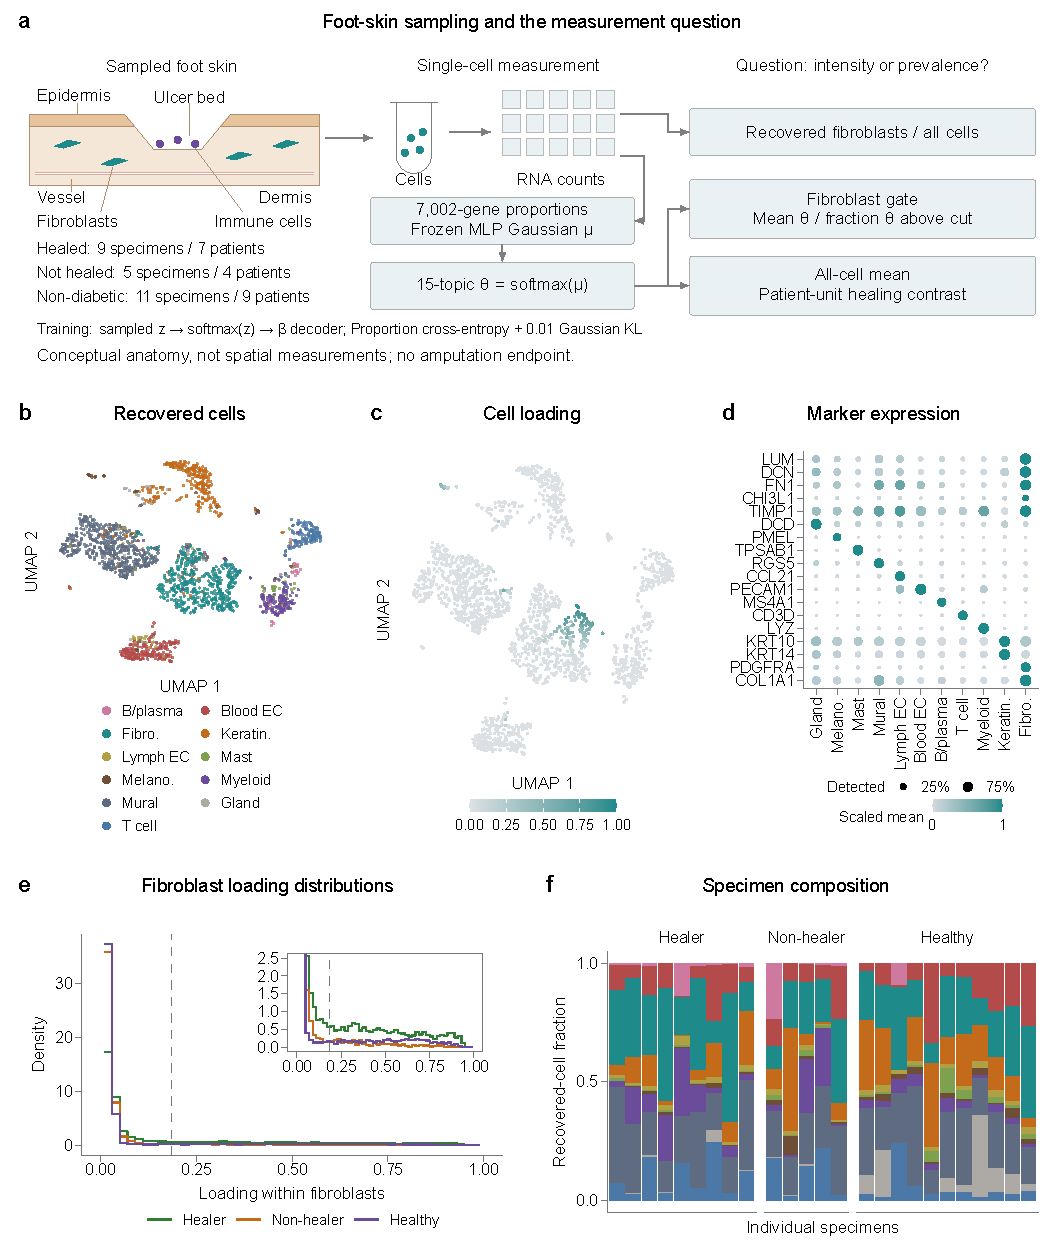
\includegraphics[width=\linewidth]{journal-figures/paper1_figure1_workflow.pdf}
\caption{What is measured in diabetic-foot skin? (a) Conceptual foot skin and destructive sampling, not measured histology. The 25 specimens represent 7 healed, 4 non-healed and 9 non-diabetic people. Composition uses recovered-cell counts; frozen inference maps 7,002-gene proportions through Gaussian mean μ to 15-topic softmax θ. Fibroblast mean/fraction and the all-cell patient mean are separate summaries. Neither readout feeds the other. Training: sampled z, normalized decoder β, cross-entropy plus 0.01 Gaussian KL. No amputation endpoint is measured. (b) Uniform display of 2,000 of 76,461 cells by marker-derived lineage; Fibro., fibroblast; EC, endothelial; mural, pericyte/smooth muscle. (c) The same cells by loading. (d) Expression: size is detection fraction, color gene-wise scaled mean log-normalized expression. Annotation markers are not independent label validation. (e) All 19,410 fibroblast loadings with the original cut; inset expands density 0--2.5, preserving the spike. (f) Composition in 25 specimens; colors match b. Non-diabetic people lack healing outcomes; inference uses full data and patient units.}\label{fig:p1f1}\end{figure}

Raw-count reconstruction reproduced all saved lineage assignments and their sample order. The measured marker profiles provide an expression-level view of those assignments and of the programme-associated genes (Figure~\ref{fig:p1f1}d). Loading distributions within fibroblasts retain both low and high values across the clinical groups (Figure~\ref{fig:p1f1}e), while individual specimens differ in their recovered cell composition (Figure~\ref{fig:p1f1}f).

Cohort roles and patient-level tissue measurements are detailed in Supplementary Table~S1 and Supplementary Table~S21.

\subsection{The frozen representation is structured, but its principal loading is a mixture coordinate}
The discovery representation retained 76,461 quality-controlled cells from 25 selected foot-skin samples in the original 54-sample series. Beta perplexity was 243, and the manifold audit passed its recorded integrity checks. The connectivity statistic in Supplementary equation~(S1) does not establish local geometric fidelity. The fitted loss in Equation~\eqref{eq:p1loss} uses Gaussian sampling and regularization as specified in Equation~\eqref{eq:p1gaussian}; deterministic readouts use the encoder mean, not a newly sampled latent state. Fibroblast topic was enriched for TIMP1, COL3A1, DCN, FN1, LUM and CHI3L1, with immediate-early and oxidative-stress genes also present among the top-ranked terms. The gene list therefore supports a fibroblast-associated inflammatory/stress description; it does not by itself establish a unique cell state or a healing mechanism.

Applying the mean--fraction identity in Equation~\eqref{eq:p1identity} to all 19,410 discovery fibroblasts clarified the remaining within-bin contribution.

A historical exploratory scan of 31 covariates across 25 specimens yielded 14 numerical BH q values below 0.05 under a naive independent-row analysis.

Recomputing all 31 covariates after denominator-specific aggregation to 20 patients retained descriptive correlations of 0.859 with B/plasma-cell fraction, $-0.765$ with the CFD/APOD-rich mean, 0.772 with PTPRC positivity and 0.662 with the fibroblast-count-weighted average of specimen median UMI counts.

The saved six-fit diagnostic does not replace the discovery fit or its patient readouts.

Only the inherited-panel 40,000-step seed-0 fit passed the training plateau screen; no fit passed its held screen.

\FloatBarrier
The hard-threshold fraction in Equation~\eqref{eq:p1fraction} uses a pooled two-Gaussian fit for a descriptive threshold; this fit did not test a continuous-shift model against a biological mixture model. Across the 25 analyzable samples, the sample mean and hard-threshold high-state fraction had Spearman $\rho=0.933$ (Figure~\ref{fig:p1f2}a\label{call:p1f2}).

\begin{figure}[tbp]\centering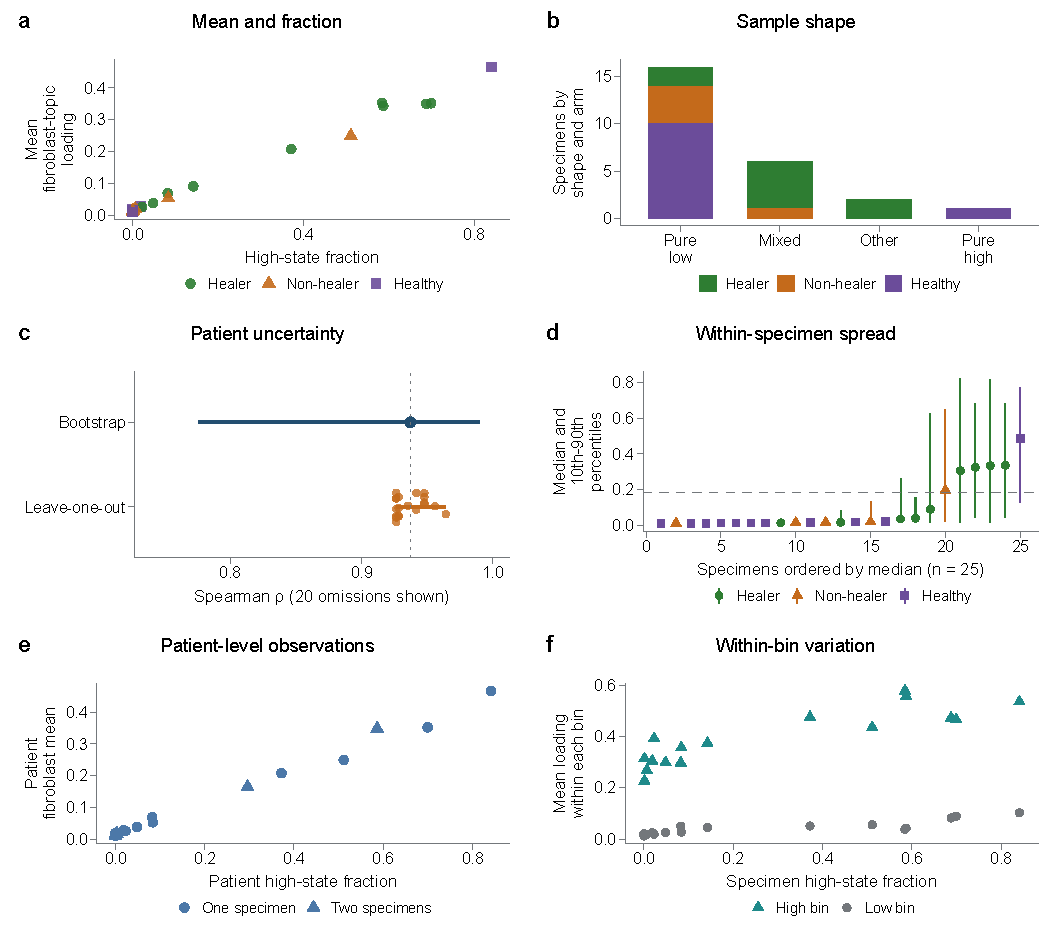
\includegraphics[width=\linewidth]{journal-figures/paper1_figure2_mixture_semantics.pdf}
\caption{Mean, prevalence and within-bin variation. (a) The 25 specimens comprise 9 healing, 5 non-healing and 11 non-diabetic samples; the cut is 0.1842958 and Spearman ρ=0.933. (b) Stacks retain clinical-arm composition in quantile-defined shapes: pure low has the 90th percentile at most 0.15, pure high the 10th percentile at least 0.10, and mixed the 10th percentile at most 0.05 and 90th percentile at least 0.40. (c) After fibroblast-count pooling to 20 patients, ρ=0.937; blue is the saved patient-bootstrap 95\% interval, while orange shows all 20 omission estimates and their range. Vertical jitter separates identical correlations. (d) Ordered specimen medians and 10th--90th percentiles are loading distributions, not confidence intervals. (e) All 20 patient means and fractions; symbols identify one or two contributing specimens, not outcome groups. (f) Low- and high-bin means against specimen high fraction; undefined empty-bin means are not plotted. These shared-cell summaries do not identify discrete biological states, constant component intensities or a healing effect.}\label{fig:p1f2}\end{figure}



Quantile-based sample categories summarize the coexistence of low and high loadings without assigning a biological mechanism to those categories (Figure~\ref{fig:p1f2}b). Omitting one patient at a time gave correlations of 0.927--0.964 (Figure~\ref{fig:p1f2}c; Supplementary Table~S16).

The median and 10th--90th percentile ranges preserve the within-specimen loading spread behind the shape categories (Figure~\ref{fig:p1f2}d).

The complete patient-level mean--fraction scatter retains all 20 mapped patients and distinguishes one from two contributing specimens (Figure~\ref{fig:p1f2}e). Low- and high-bin means vary across specimens when the corresponding bin contains cells (Figure~\ref{fig:p1f2}f).

Mixture-coordinate and exploratory covariate associations are detailed in Supplementary Table~S8 and Supplementary Table~S10.

\subsection{The operational high-state pattern survives selected technical controls}

The operational high-state pattern survived the originally specified artifact challenges, while the expanded controls identify measurement dependence.

The unchanged-label count match and the alternative marker gate address different perturbations: the former reduces counts within an existing cell set, while the latter changes assignments. \FloatBarrier
The stress and PTPRC challenge ratios are displayed relative to their prespecified rejection bounds (Figure~\ref{fig:p1f3}a\label{call:p1f3}), whereas the matched-depth scatter retains individual specimen fractions rather than a single agreement statistic (Figure~\ref{fig:p1f3}b).

\begin{figure}[tbp]\centering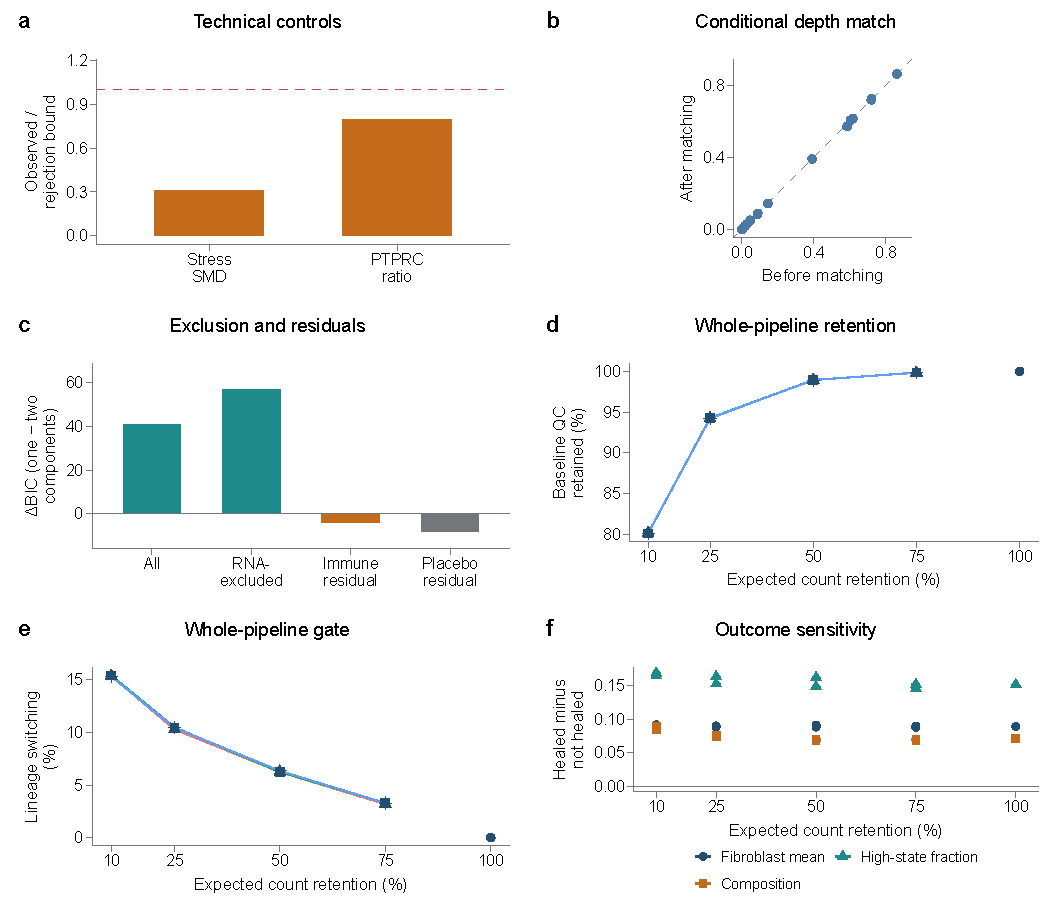
\includegraphics[width=\linewidth]{journal-figures/paper1_figure3_artifact_controls.pdf}
\caption{Conditional controls and whole-pipeline sensitivity. (a) Stress SMD and PTPRC rate ratio divided by their rejection bounds; dashed line: one. (b) Specimen fractions before and after matching 14,561 eligible fibroblasts to 986 panel counts; identity is dashed. The 99.5\% agreement conditions on original lineage labels. (c) One-minus-two-component BIC for 24 matched specimens before and after immune-transcript exclusion, and separately for immune- and placebo-covariate residuals in 25 specimens. Both residual comparisons favor one component; their samples and perturbations are not interchangeable. (d) Retention of baseline QC survivors after count thinning and rerunning QC. (e) Lineage switches among common survivors. d/e retain all three computational seeds and the unthinned baseline. (f) Seed minima and maxima of patient contrasts for three readouts; these ranges are sensitivities, not confidence intervals. The same 7 healed and 4 non-healed patients, frozen gate, encoder and cut are used. Conditional stability does not establish whole-pipeline invariance, identity truth or clinical portability.}\label{fig:p1f3}\end{figure}



Whole-pipeline perturbations expose losses of baseline QC cells (Figure~\ref{fig:p1f3}d) and changing lineage assignments among shared survivors (Figure~\ref{fig:p1f3}e). The ranges of patient contrasts across these same perturbations are shown separately (Figure~\ref{fig:p1f3}f), so persistence of a contrast is not mistaken for stability of the cells entering its denominator.

The full released-count audit reproduced the 81,602 pre-QC cells, 76,461 baseline survivors and all 19,410 fibroblast assignments, with a maximum deterministic-coordinate discrepancy below $4.77\times10^{-7}$.

Removing cells carrying any of the prespecified immune transcripts left the specimen high-state fractions nearly unchanged ($\rho=0.989$) and increased the BIC support for two components fitted to the sample fractions (Figure~\ref{fig:p1f3}c).

Transcript exclusion, the depth audit and its outcome comparisons are detailed in Supplementary Table~S11, Supplementary Table~S30 and Supplementary Table~S31.

\subsection{High-state abundance does not establish healing specificity}

The lineage marker list shared no genes with the specified top-gene list used to describe the tested topic.

The high-state pattern was not restricted to samples labelled as healing.

For the separate all-cell mean-loading contrast in Equation~\eqref{eq:p1delta}, collapsing repeats to 11 patients gave a healing-minus-non-healing difference of 0.0293.

The specimen-level arm fractions display the non-diabetic counterexample (Figure~\ref{fig:p1f4}a\label{call:p1f4}). The all-cell contrast display separately retains specimen- and patient-unit intervals, with patient-omission points showing influence rather than extra outcomes (Figure~\ref{fig:p1f4}b).

\begin{figure}[tbp]\centering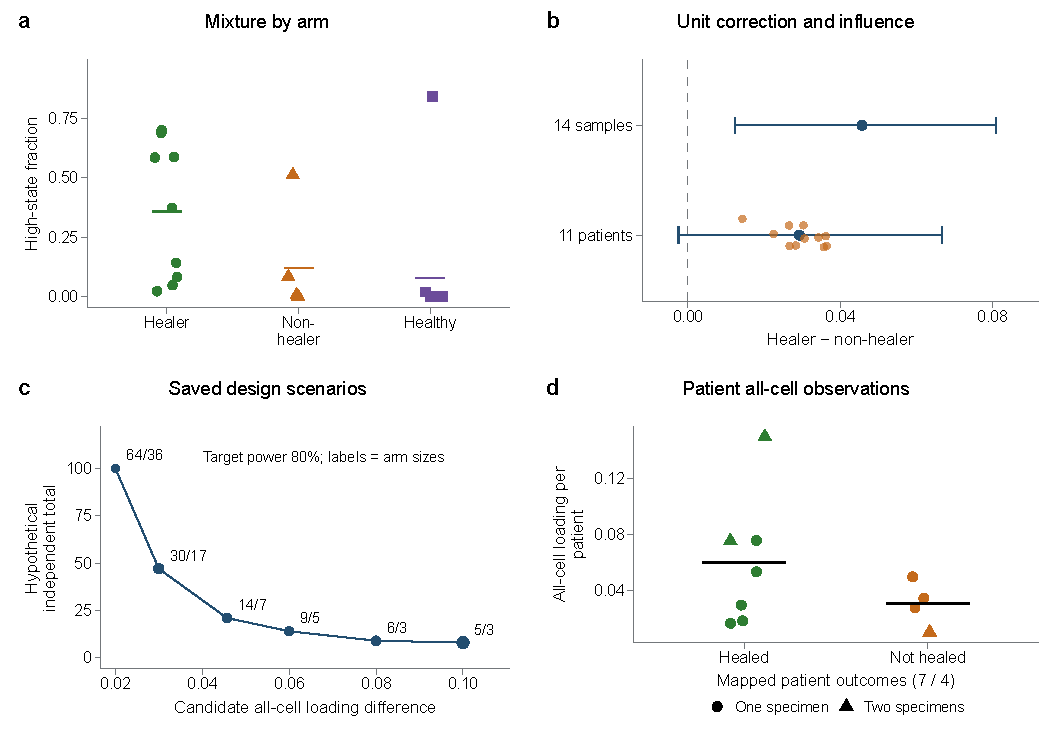
\includegraphics[width=\linewidth]{journal-figures/paper1_figure4_outcome_counterexample.pdf}
\caption{State abundance, analysis unit and saved design scenarios. (a) High-state fractions for 9 healing, 5 non-healing and 11 healthy specimens, with arm means. The healthy maximum 0.841 challenges exclusivity to healing ulcers. (b) All-cell mean-loading effects and bootstrap 95\% intervals for 14 specimens versus 11 patients; orange points retain all 11 patient omissions, not additional outcomes. (c) Six previously calculated all-cell loading-difference scenarios targeting 80\% power; labels show hypothetical healed/non-healed arm sizes. The specimen-derived spreads and independent-observation assumption are not patient-population variance estimates. These scenarios differ from the historical 24.9\% power calculation for a 9-versus-5 high-state-fraction design and are not clinical minimum important differences. (d) All-cell scores of the 7 healed and 4 non-healed patients, with arm means and symbols for one or two contributing specimens. a and d have different cell denominators; none of these displays supplies independent prognostic validation.}\label{fig:p1f4}\end{figure}



Patient scores, equivalence sensitivity and the DFU-only null are detailed in Supplementary Table~S2, Supplementary Table~S15 and Supplementary Table~S27.

\subsection{Retrospective design simulations do not resolve outcome uncertainty}

A retrospective simulation substituted the observed specimen-level high-state-fraction effect and pooled spread into a hypothetical 9-versus-5 independent-specimen design, giving 24.9\% estimated power.

We also ran a design calculation for the next cohort, keeping it separate from the biological results.

The six saved difference-detection scenarios are shown together rather than as an isolated power bar (Figure~\ref{fig:p1f4}c). The original 11 patient all-cell values and contributing specimen counts remain separately visible (Figure~\ref{fig:p1f4}d), without equating a hypothetical design with observed outcomes.

Because repeated biopsies do not add outcomes, the fibroblast readouts were next summarized for each patient, together with their sampling and influence sensitivities (Figure~\ref{fig:p1f5}a--h\label{call:p1f5}).

\begin{figure}[tbp]\centering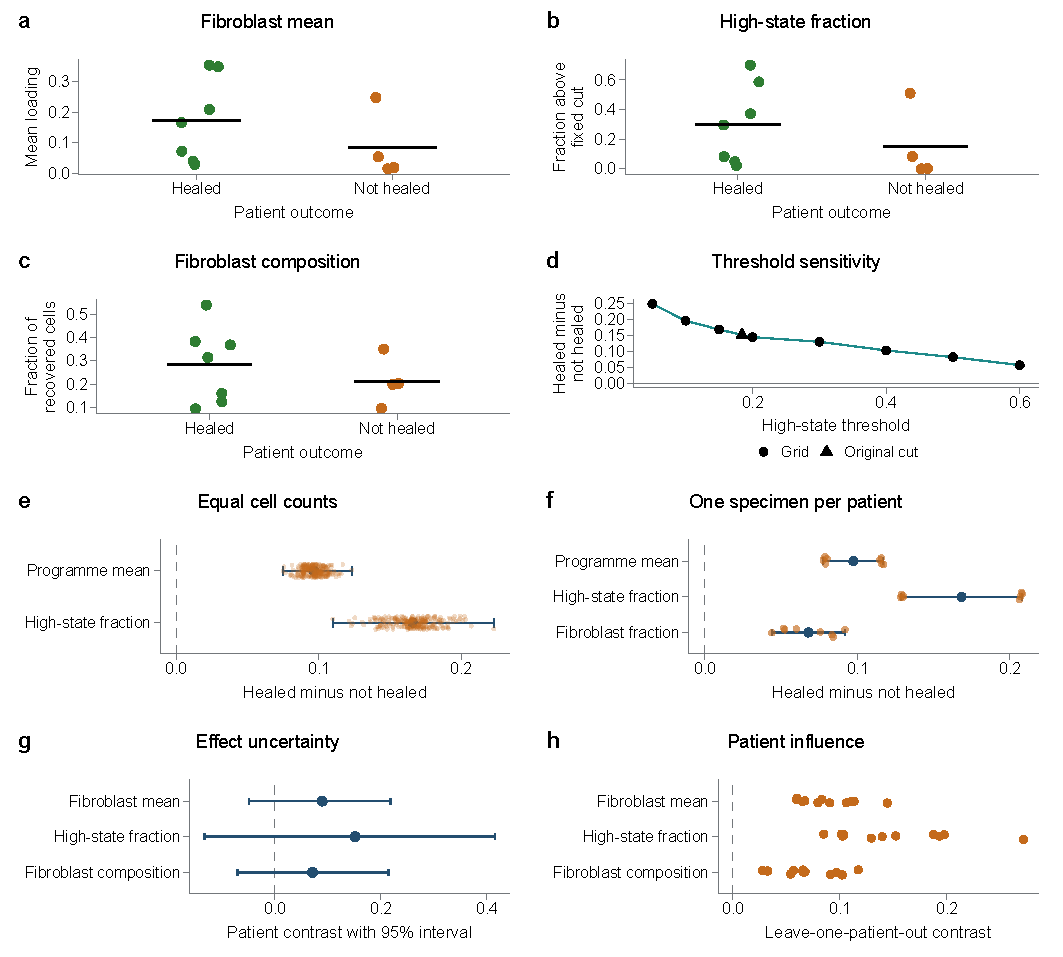
\includegraphics[width=\linewidth]{journal-figures/paper1_figure5_patient_readouts.pdf}
\caption{Patient-unit readouts, uncertainty and influence. a--c show 7 healed and 4 non-healed DFU patients, with group means; repeated specimens are pooled using the relevant cell counts. (a) Mean fibroblast loading: difference 0.0892, exact p=0.3121. (b) Fraction above the frozen cut: difference 0.1514, p=0.3697. (c) Fibroblast fraction: difference 0.0708, p=0.4697. Tests use all 330 label allocations; BH q=0.4697 for all three. (d) High-state contrasts across eight fixed cuts and the original midpoint. (e) All 250 saved equal-cell draw contrasts, their means and full ranges, using 100 fibroblasts per specimen. (f) All eight one-specimen-per-patient choices, with means and full ranges. Vertical jitter separates saved values without changing their contrasts. (g) Cell-count-weighted effects with 10,000-draw patient-bootstrap 95\% intervals; all span zero. (h) All 11 patient omissions per readout. e, f and h describe the same patients, not confidence intervals or independent replications; positive omission estimates and intervals spanning zero can coexist without validating prognosis or equivalence.}\label{fig:p1f5}\end{figure}

The AUC planning grid is detailed in Supplementary Table~S7.

\subsection{Fibroblast-restricted patient comparisons retain substantial uncertainty}



We next evaluated the two fibroblast-restricted readouts at the same independent patient unit used for the all-cell analysis (Figure~\ref{fig:p1f5}a and~b).

Equal weighting of repeated specimen summaries within each patient gave differences of 0.0974, 0.1683 and 0.0679 for the programme mean, high-state fraction and fibroblast composition, respectively.

Individual patient loadings and high-state fractions retain the observed spread within each outcome group (Figure~\ref{fig:p1f5}a and~b).

The three patient-bootstrap intervals all cross zero (Figure~\ref{fig:p1f5}g). In contrast, every leave-one-patient-out point estimate remains positive (Figure~\ref{fig:p1f5}h).

Fibroblast composition was evaluated separately, retaining all recovered cells as its denominator. The patient-level fractions were 0.2825 and 0.2118, a difference of 0.0708 with interval $[-0.0708,0.2146]$ and $p=0.4697$ (Figure~\ref{fig:p1f5}c).

The threshold-free patient distribution statistic in Equation~\eqref{eq:p1ecdf} was 0.3045, with exhaustive $p=0.1848$ over 330 patient-label allocations. Across the eight fixed cuts and the original midpoint, high-fraction differences remained positive (0.0570--0.2485); all unadjusted probabilities exceeded 0.22 and all support-wide max-statistic probabilities exceeded 0.31 (Figure~\ref{fig:p1f5}d; Supplementary Table~S23).

Equalizing each specimen to 100 sampled fibroblasts left the programme-mean contrast positive in all 250 draws (0.0749--0.1233) and the high-state contrast positive in all draws (0.1098--0.2229); their smallest exact probabilities were 0.1273 and 0.1515 (Figure~\ref{fig:p1f5}e). Selecting one specimen per patient in all eight possible combinations gave programme-mean, high-state and composition ranges of 0.0777--0.1170, 0.1284--0.2081 and 0.0440--0.0918, respectively (Figure~\ref{fig:p1f5}f; Supplementary Table~S24).

Direct comparison of the five repeated-specimen pairs, including three DFU patients, showed that within-specimen cell partitioning does not describe all between-specimen variation.

All three patient-unit contrasts are detailed in Supplementary Table~S22.

\subsection{Method constants expose both stable and fragile claims}


The mean-versus-weight association remained positive across the cut grid, from $\rho=0.909$ to 0.948 (Supplementary Fig.~S1\label{call:p1f6}), and across K=10, 15 and 20, from $\rho=0.924$ to 0.947 (Supplementary Fig.~S1).

The healthy-skin counterexample was more conditional.

The healing-arm p value moved between 0.042 and 0.062 over the cut grid, with only 4 of 18 cuts below 0.05 (Supplementary Fig.~S1; Supplementary Table~S18 and~S17).

Tracked-topic capacity comparisons are detailed in Supplementary Table~S17.

\subsection{Negative controls and representation comparisons constrain interpretation}

The DFU-only label-permutation calibration used the 9 healing and 5 non-healing specimens, excluding all 11 healthy controls before allocation. Its observed high-state-fraction difference was +0.2380, with a central 95\% null interval {[}−0.3167, +0.3222{]} and exact $p=0.1199$ over 2,002 allocations (Supplementary Fig.~S1). The shuffle therefore reduced coordinate concentration while also narrowing row-wise library-size and detection-rate variation; because it does not preserve row-wise library sizes, it is a co-expression-structure control rather than a complete technical null (Supplementary Fig.~S1; Supplementary Table~S25). In the anatomical permutation control, the observed p value was 0.0015 and 5.0\% of permuted comparisons fell below 0.05 (Supplementary Fig.~S1).

The historical specimen-level scoring procedure used the pairwise AUC statistic in Equation~\eqref{eq:p1auc} and gave point AUCs of 0.822 for fibroblast-associated topic, 0.844 for the module score, 0.533 for PCA and 0.878 for NMF. They document the earlier procedure rather than supply evidence for a representation ranking (Supplementary Fig.~S2\label{call:p1f7}; Supplementary Table~S3, S5 and~S13).

The sample-level readouts had pairwise Spearman correlations from 0.174 to 0.710 (Supplementary Fig.~S2).



Paired pooled-score AUC differences are detailed in Supplementary Table~S13.

\subsection{Same-model patient-pair discrimination and paired anatomical sensitivity}

The revised held-pair statistic in Equation~\eqref{eq:p1pairauc} evaluated all 28 healing/non-healing pairs from the 11 patients, fitting each scoring rule on the other nine patients.

The earlier leave-one-patient-out procedure remains separately documented: topic AUC was 0.714 with add-one permutation $p=0.2991$, module AUC was 0.786 with $p=0.166$, PCA was 0.500 and NMF was 0.125.



The scoring-rule summary (Figure~\ref{fig:p1f8}a\label{call:p1f8}) is complemented by the complete pair-level win, tie and loss display, retaining all 28 dependent comparisons (Figure~\ref{fig:p1f8}c). Individual tissue pairs likewise show the dispersion behind the anatomical mean (Figure~\ref{fig:p1f8}d); neither display increases the number of independent patients.

\begin{figure}[tbp]\centering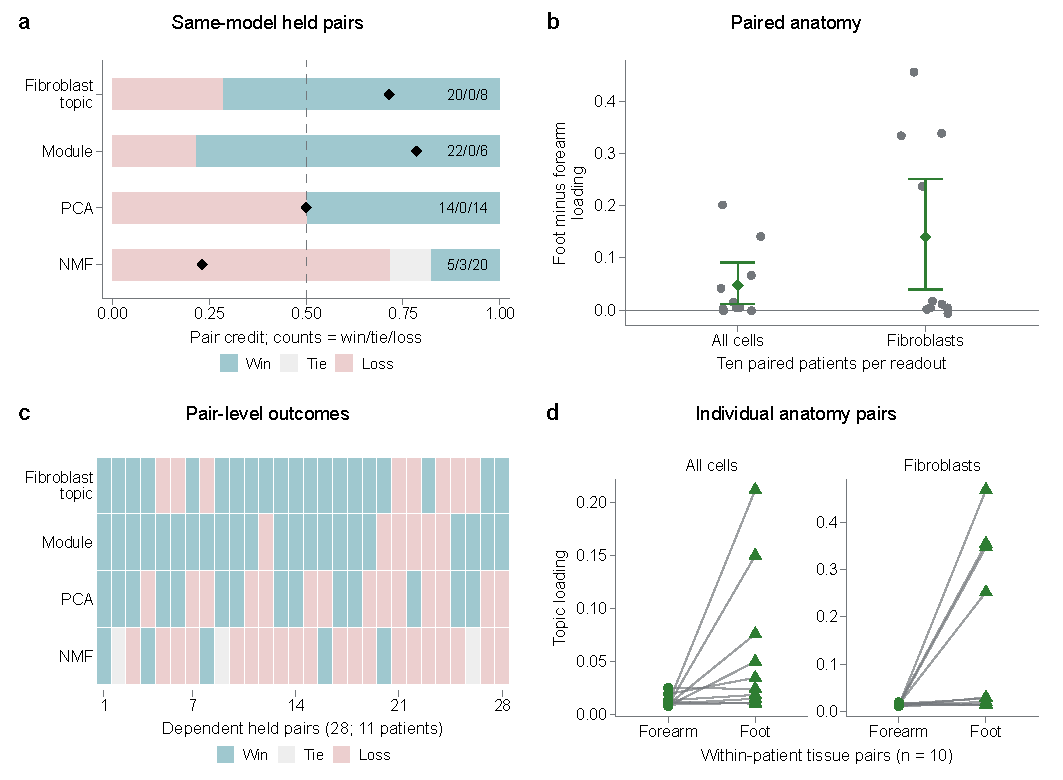
\includegraphics[width=\linewidth]{journal-figures/paper1_figure8_patient_unit_anatomy.pdf}
\caption{Patient-pair discrimination and anatomical sensitivity. (a) Win/tie/loss fractions and counts for each scoring method, with a black diamond at its mean credit across 28 held pairs. Every fold fits on the other nine patients; ties earn half credit. The pairs share 7 healed and 4 non-healed patients and have no binomial confidence interval. (b) All 10 paired foot-minus-forearm differences for both all-cell and fibroblast-restricted loading, overlaid with saved means and paired-patient bootstrap 95\% intervals. For the all-cell topic, sign-flip p=0.0107 and BH q=0.0402. (c) All dependent held-pair wins, ties and losses in saved order. (d) The same 10 patients' forearm and foot levels, separately for the two cell denominators with distinct vertical scales. b and d are different summaries of the same pairs, not 20 independent people. Neither this anatomical sensitivity nor the shared-patient scoring comparison supplies independent clinical validation.}\label{fig:p1f8}\end{figure}

Across 10 paired patients, the fibroblast-associated topic was higher in foot than in forearm skin by +0.0476 (exhaustive sign-flip $p=0.0107$, BH $q=0.0402$); the fibroblast-restricted contrast was +0.1398 ($p=0.0146$). Four of 15 topics remained significant after BH correction (Figure~\ref{fig:p1f8}b; Supplementary Table~S14).

Pooled diagnostics and revised held-pair results are detailed in Supplementary Table~S4 and Supplementary Table~S29.

\subsection{External projections remain construct audits}

A separate projection into GSE231643 provides a weaker, label-only concordance of direction: the within-fibroblast ratio falls from 2.89 in the discovery analysis to 1.66 (sample-bootstrap 95\% interval 1.01--6.10; two-sided Mann--Whitney $p=0.1429$; Supplementary Table~S12).

The external immune-axis analysis used mutually exclusive lineage compartments.

GSE268834 supplied another descriptive projection: the topic-associated fibroblast signal correlated with exclusive immune fraction at +0.714, and the diabetic-minus-non-diabetic fibroblast-topic contrast was +0.0464 with $p=0.2812$.

GSE248247 was a deliberately low-yield stress test of the frozen projection.

Across these projections, immune-axis correlations, library-complexity associations and diabetic/non-diabetic contrasts target different estimands and stay cohort-specific.

\Needspace{6\baselineskip}
The cohort correlations appear in Figure~\ref{fig:p1f9}a\label{call:p1f9}; lineage-share and library-complexity associations in Figure~\ref{fig:p1f9}b; and group contrasts in Figure~\ref{fig:p1f9}c. Individual immune fractions (Figure~\ref{fig:p1f9}d), detected-gene summaries (Figure~\ref{fig:p1f9}e) and diabetic/non-diabetic specimen values (Figure~\ref{fig:p1f9}f) retain the observations underlying those summaries.

\begin{figure}[tbp]\centering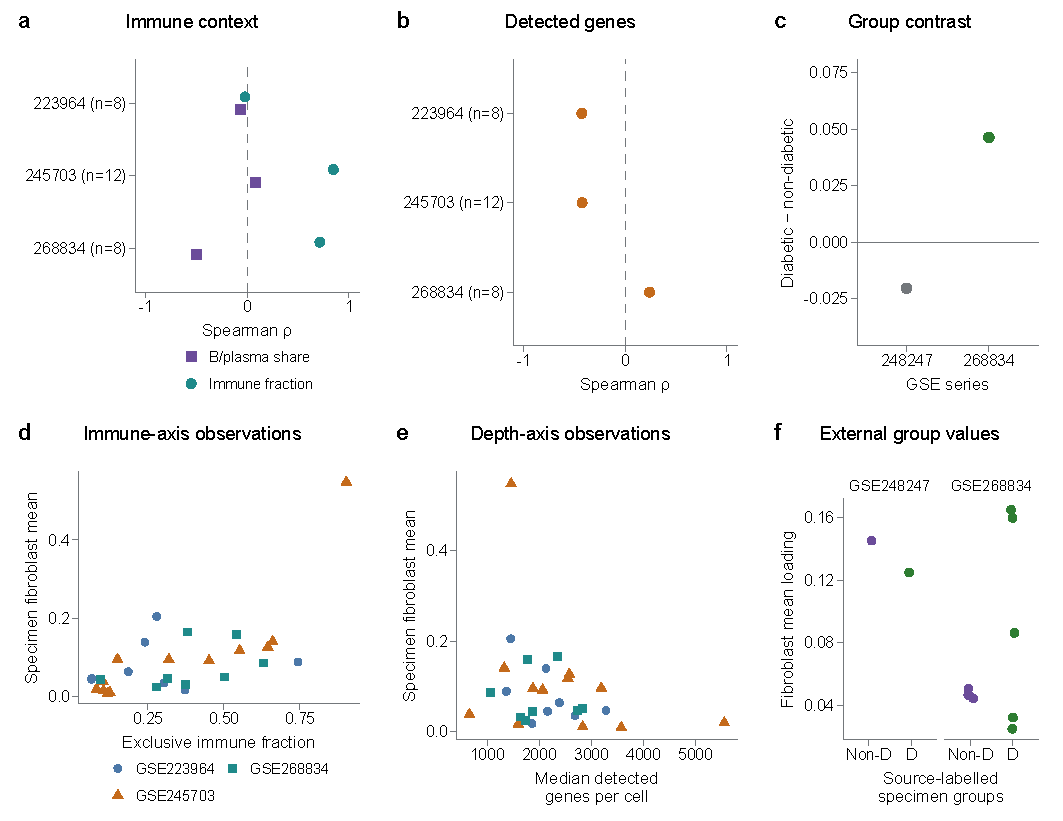
\includegraphics[width=\linewidth]{journal-figures/paper1_figure9_external_construct_audit.pdf}
\caption{External tissue-context projections, not healing validation. (a) Saved correlations with exclusive immune fraction and B/plasma share. (b) Saved correlations with median detected genes per cell. (c) Diabetic-minus-non-diabetic fibroblast contrasts: +0.0464 in GSE268834 and −0.0204 in GSE248247. (d) All specimen fibroblast means against exclusive immune fractions in the three cohorts (8, 12 and 8 specimens). (e) The same observations against median detected genes per cell. (f) Individual source-labelled diabetic and non-diabetic specimen values in the two group comparisons; GSE248247 has only one specimen per group. Correlations and raw points summarize the same data, not separate replications. Gene coverage, tissue sampling and cell yields differ, authoritative healing outcomes are absent, and no biological confidence intervals are inferred.}\label{fig:p1f9}\end{figure}



External sample-level correlations are detailed in Supplementary Table~S9.

\subsection{Patient restriction and saved-fit pooling distinguish the remaining audit units}

Restriction to the same 11 DFU patients changed several descriptive associations without adding patients or an outcome test. The mixed-patient display in Figure~\ref{fig:p1f2}e is not an independent DFU-only validation.

The saved pooling bridge retained all six topic/cut contracts and 120 patient--fit rows, with the same 16 training and four held patients in every fit (Supplementary Table~S36 and~S38). Pooling corrects an estimand mismatch; it does not reproduce independent patients, resolve inherited preprocessing/reference dependence or replace the primary discovery outcome values in Figure~\ref{fig:p1f5}a--c.

\subsection{Capacity and initialization distinguish measurement association from programme identity}

All nine fixed 40,000-step fits and their full checkpoint projections passed replay, with zero maximum absolute projection discrepancy. Primary one-to-one decoder correlations ranged from 0.6038 to 0.9876, whereas the specimen mean--fraction association remained high at $\rho=0.9060$--0.9503 (Supplementary Fig.~S3\label{call:p1f10}; Supplementary Table~S39). The all-topic display retains 120 assigned reference correlations and all 15 capacity-limited reference omissions rather than substituting rowwise best matches (Supplementary Fig.~S3); the full numerical matching table also retains the 15 unmatched new topics.



All 240 person-specific computational range rows contained three estimable seeds. The largest within-K fibroblast-only widths were 0.2774 for mean loading and 0.3647 for the fraction above the descriptive cut (Supplementary Fig.~S3; Supplementary Table~S41); the readouts were therefore not uniformly seed-insensitive. For M1 versus C1, specimen-median held-cell log-score differences were positive in every fit (0.0949--0.2513 nats/cell), but person-specific differences spanned $-0.5625$ to 1.1232 and only 13--16 of the existing 20 people favored M1 in a given fit (Supplementary Fig.~S3; Supplementary Table~S40).

\subsection{Topic selection, tissue context and the composition of the mean}

Repository records show that topic 0 was named after the per-arm topic means of the discovery fit were inspected, when it had the largest healed/non-healed ratio of the 15 topics. The observed all-cell ratio of topic 0 (1.96) was smaller than the median largest ratio under random labels (2.28), giving a maximum-calibrated p of 0.785 (Figure~\ref{fig:p1f11}a\label{call:p1f11}); the corresponding values for named topic 0 were 0.609 for the fibroblast mean and 0.955 for fit-specific topic-cut fractions.

\begin{figure}[tbp]\centering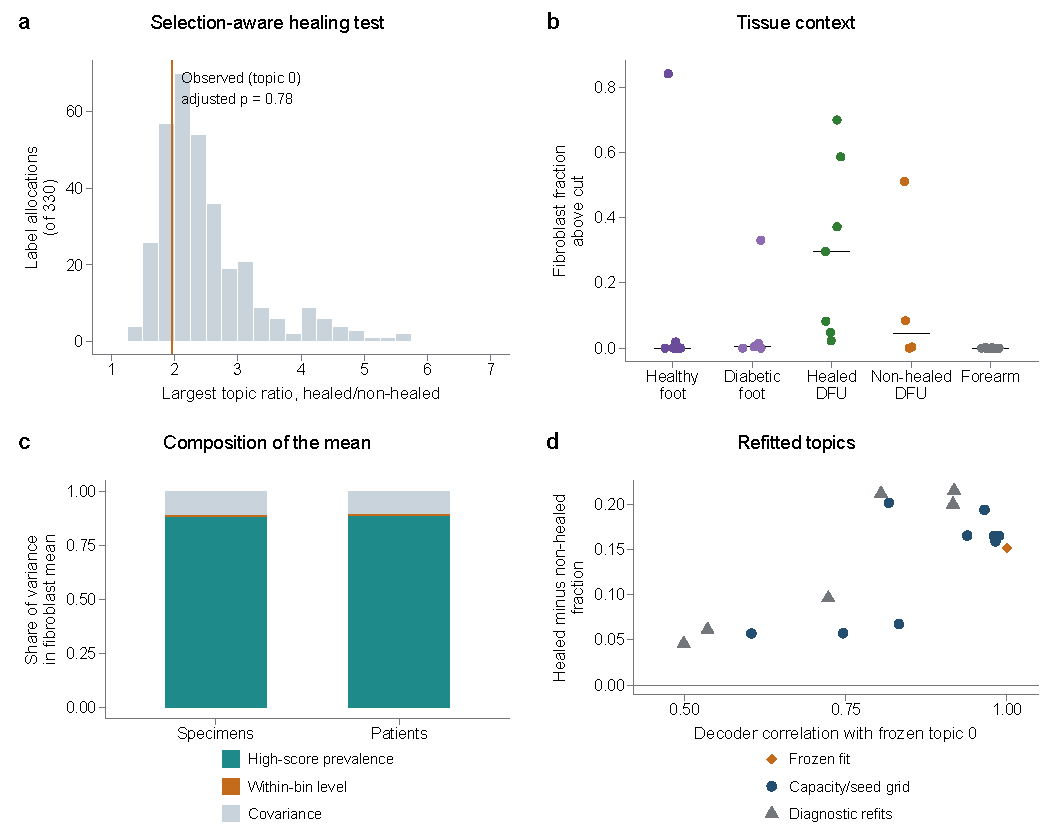
\includegraphics[width=\linewidth]{journal-figures/paper1_figure11_selection_context.pdf}
\caption{Selection, tissue context and composition of the fibroblast readout. (a) Each of the 330 allocations of 7 healed among the 11 DFU patients gives the largest healed/non-healed all-cell mean ratio over the 15 topics; the orange line is the observed ratio of topic 0, which was named after its arm-wise means were inspected, and the adjusted p is the fraction of allocations at least as extreme. (b) Patient-level fraction of fibroblasts above the frozen cut in intact healthy and diabetic foot skin, healed and non-healed ulcers, and forearm skin from all groups; bars are medians. (c) Shares of between-unit variance in the fibroblast mean from the high-score prevalence term, the within-bin level term and their covariance in the exact mean decomposition. (d) Healed minus non-healed fraction of fibroblasts above the topic cut for the frozen fit and 15 refits, each scored with its own matched topic and cut, against the decoder correlation of that topic with frozen topic 0; no refit gives an exact permutation p below 0.05.}\label{fig:p1f11}\end{figure}

The excluded intact foot-skin specimens from diabetic donors and the forearm specimens were projected through the frozen pipeline (Figure~\ref{fig:p1f11}b).

The exact mean decomposition was quantified directly (Figure~\ref{fig:p1f11}c).

Finally, the healing contrast was recomputed for each of the nine capacity/seed refits and six diagnostic refits, using each fit's own matched topic and cut (Figure~\ref{fig:p1f11}d).



\subsection{Clinical balance and an independent bulk wound score}

Age, sex, BMI, HbA1c, wound area and diabetes duration were compared within the same 11 DFU patients (Supplementary Table~S42).

Three frozen decoder scores were then evaluated in 12 independent bulk foot samples, six ulcers and six intact-skin samples, on the full mapped array (Supplementary Table~S44).

Readout associations with clinical covariates are detailed in Supplementary Table~S43.

\section{Discussion}

The frozen fibroblast readout is enriched in the sampled ulcers, and its mean is dominated by high-score prevalence under the chosen cut. The prevalence term contributed close to nine-tenths of between-specimen and between-patient variance, while within-bin levels and their covariance also contributed.

The nine-fit capacity and initialization audit sharpens the distinction between a measurement association and a reproducible programme identity. Mean--fraction correlations remained high while decoder matches, loading cuts and some person-specific readouts varied substantially.

The patient-unit extension connects the fibroblast interpretation directly to the available healing categories. Averaging programme scores within fibroblasts, counting high-scoring fibroblasts and counting fibroblasts among all cells all gave higher point estimates in healed patients, but each comparison retained considerable uncertainty.

The different uncertainty summaries answer different questions. Patient bootstrap intervals resample the observed outcome arms and inherit the limitations of their small empirical distributions \citep{efron1993}.

The cell atlas and expression profiles also clarify what is still missing experimentally. Melanocytes carried the highest loading, so the score is not a count of one anatomically defined fibroblast population, and doublet removal left the contrasts unchanged.

This distinction has biological consequences. A high mean could accompany recruitment or recovery of a particular fibroblast population, increased expression within an existing population, or changes in several populations at once.

The threshold should be understood as an operational convention. It permits a reproducible high-state fraction and makes the denominator explicit, while assigning nearby scores on opposite sides of the cut to different bins.

The technical controls provide evidence about selected perturbations of this operational measurement. Most state labels survived count matching under fixed lineage assignments, and specimen fractions were stable after specified immune-transcript exclusions.

The difference between a tissue measurement and a healing predictor becomes clearer at the patient level. One healthy specimen had the highest fraction. High-scoring fibroblasts met the presence rule in 2 of 15 intact-foot donors, so the readout is neither specific to diabetes nor categorically absent from intact skin.

The representation comparison remains an internal audit. Historical pooled-fold PCA and NMF coordinates are not directly comparable across fitted models, and their bootstrap contrasts cannot establish representation quality.

The separate budget and training-panel fits distinguish optimization sensitivity from clinical validation. Longer fits reduced decoder similarity and reconstruction error within the inherited panel, but most training screens and all held screens failed the fixed engineering plateau rule.

Even reliable discrimination would leave other clinical questions unanswered. AUC describes ordering of outcomes, whereas calibration concerns whether predicted risks agree with observed risks in the population where the model is used \citep{steyerberg2010,vancalster2019}.

The paired foot--forearm contrast illustrates the importance of sampling context. Half of its foot specimens were ulcers, and one of the five intact-foot pairs had a large high-score fraction.

An independent bulk foot series, with no healing labels, gave a higher topic-specific gene score in ulcers than in intact skin and no corresponding separation of diabetic from non-diabetic intact skin. The genes with the largest decoder weights, and a weight taken over the whole overlapping panel, remained compatible with exchange of those sample labels.

Future evaluation needs a defined outcome horizon, fixed sampling and readout, and a prespecified prognostic estimand. Amputation was not an evaluated endpoint, so this audit cannot estimate amputation risk or support amputation-related treatment decisions.

\section*{Additional Information}
Funding. No funding was received for this study.

Competing interests. The author declares no competing interests.





Consent for publication. The article contains no identifiable individual information or participant images. The tissue drawings are conceptual illustrations.

\section*{Data Availability}
Public processed counts and annotations are available from NCBI Gene Expression Omnibus under GSE165816, GSE231643, GSE241132, GSE223964, GSE245703, GSE268834, GSE248247 and GSE80178. Numerical tables accompany this article; the study repository's Releases page provides the current versioned reproduction package, including derived results, frozen models, editable figures and acquisition instructions. Its reproduction scope is stated below. No request to the author is required. Raw GSE165816 sequencing reads remain restricted by source-study participant privacy; unreleased patient identifiers and individual closure times are not imputed.

\section*{Code availability}
Current analysis software, numerical evidence, saved evaluation inputs and reproduction instructions are available at \url{https://github.com/PeterPonyu/wound-measurement-construct} and archived at software DOI \url{https://doi.org/10.5281/zenodo.23308073}. The archive manifest identifies the included checkpoints and analysis records. Source-study inputs retain their original terms.

The current archive includes the revised analyses and documented saved-state evidence. Earlier immutable archives identify earlier software releases. Document reconstruction, verification of saved numerical evidence and fresh model fitting are separate tasks; full fitting requires the specified upstream inputs and computing environment. No additional biological replication is claimed by packaging.

Acknowledgements. The author thanks the original investigators and participants for making the source datasets available.
\FloatBarrier
\bibliographystyle{unsrtnat}
\bibliography{references_paper1}

\section*{Author contributions}
Zeyu Fu conceived the study, developed the methodology and software, curated the public data, performed and verified the analyses, prepared the visualizations, and wrote and revised the manuscript.

\end{document}